\documentclass[../../manuscript.tex]{subfiles}

\begin{document}

\chapterimage{theory_ch_cover.png}
\chapter{Theory}\label{ch:theory}
\newpage

% sections
\section{Physical system}\label{sec:physical_system}

\subsection{Derivation of system of equations}

\subsection{Variational formulation}

\newpage
\section{Projection methods}\label{sec:projm}
This section is largely based on the extremely instructive book by \citeauthor{iter_method_saad} about iterative methods \cite[Section 5: Projection Methods]{iter_method_saad}.

Most iterative methods that aim to solve (large) linear systems like
\[
    Ax = b
\]
for $x, b \in \mathbb{R}^n$ and $A \in \mathbb{R}^{n \times n}$ a linear operator, can be interpreted as projection methods.

A general description of projection methods is as follows let $x_0 \in \mathbb{R}^n$ be an initial guess, $\mathcal{K}, \mathcal{L}$ subspaces of $\mathbb{R}^n$, $r_0 = Ax_0 - b$ the residual.
\begin{subequations}\label{eq:projm_general}
    \begin{align}
        \tilde{x}                & = x_0 + \delta, \quad \delta \in \mathcal{K} \label{eq:projm_ic_plus_correction}
        \\
        \quad (r_0 - A\delta, w) & = 0, \quad \forall w \in \mathcal{L}.
        \label{eq:projm_orthogonality_condition}
    \end{align}
\end{subequations}
where $\delta$ is the correction to the initial guess $x_0$ and $(\cdot, \cdot)$ is the inner product \cite[Equation 5.5-6]{iter_method_saad}. The second equation is the orthogonality condition.

Furthermore, orthogonal projection methods are a subclass of projection methods where $\mathcal{K} = \mathcal{L}$. The most well-known orthogonal projection method is the conjugate gradient method,  \cref{sec:cg}. In the case where $\mathcal{K} \perp \mathcal{L}$, the method is oblique projection method. Examples of oblique projection

\subsection{Matrix representation}
Let V and W be the bases for $\mathcal{K}$ and $\mathcal{L}$ respectively. Then \cref{eq:projm_ic_plus_correction,eq:projm_orthogonality_condition} can be written as 
\begin{align}
    \tilde{x} & = x_0 + Vy, \\
    W^TAVy    & = W^Tr_0.
\end{align}
In case $W^TAVy$ is invertible, the solution is \cite[Equation 5.7]{iter_method_saad}
\begin{equation}
    x = x_0 + (W^TAV)^{-1}W^Tr_0.
    \label{eq:projm_approximate_solution}
\end{equation}

\subsection{Interpretation in terms of projectors}\label{sec:projm_projectors}

\subsubsection{Residual projection methods} 
Let $\mathcal{L} = A \mathcal{K}$ and define the approximate residual
\begin{equation}
    \tilde{r} = b - A\tilde{x} = r_0 + A\delta.
    \label{eq:projm_residual}
\end{equation}
then $\tilde{r}$ is the residual is $r_0$ minus its orthogonal projection onto $\mathcal{L}$, $P_{\mathcal{L}}$. This can be expressed as \cite[Proposition 5.4]{iter_method_saad}
\begin{equation}
    \tilde{r} = r_0 - P_{\mathcal{L}}r_0 = (I - P_{\mathcal{L}})r_0.
    \label{eq:projm_residual_projection}
\end{equation}

\subsubsection{Error projection methods} 
Similarly, suppose $\mathcal{K} = \mathcal{L}$ and $A$ is SPD. Then the correction vector is obtained by constraining the residual vector $r_0 - A\delta$ to be orthogonal to $\mathcal{K}$.
\begin{equation*}
    (r_0 - A\delta, w) = 0, \quad \forall w \in \mathcal{K}.
\end{equation*}
Now, define the initial error
\begin{equation}
    e_0 = x_* - x_0
    \label{eq:projm_error_initial}
\end{equation}
and the error after approximation
\begin{equation}
    \tilde{e} = x_* - \tilde{x}.
    \label{eq:projm_error_approximation}
\end{equation}
Then,
\begin{align*}
    A\tilde{e} & = A(x_* - x_0 - \delta) \\
               & = A(e_0 - \delta)       \\
               & = r_0 - A\delta         \\
\end{align*}
Hence, the orthogonality condition can be written as
\begin{align*}
    (A\tilde{e}, w) = (e_0 - \delta, w)_{A} = 0, \quad \forall w \in \mathcal{K}.
\end{align*}
It follows that the correction vector $\delta$ is the error $e_0$ projected onto $\mathcal{K}$ with respect to the inner product $(\cdot, \cdot)_A$ \cite[Proposition 5.5]{iter_method_saad}.
\begin{equation}
    \tilde{e} = (I - P_{\mathcal{K}}^{A}) e_0.
    \label{eq:projm_error_projection}
\end{equation}

\subsection{Projection-based iterative methods (1D)}
In general these kinds of methods are invoked when $\mathcal{K} = \text{span}\{v\}$ and $\mathcal{L} = \text{span}\{w\}$ for some vectors $v, w \in \mathbb{R}^n$ and may be described by the algorithm
\begin{align*}
    r      & \leftarrow b - Ax,                 \\
    \alpha & \leftarrow \frac{(r, w)}{(Av, w)}, \\
    x      & \leftarrow x + \alpha v.
\end{align*}

\subsubsection{Steepest descent}
For the case where $A$ is SPD 
\begin{algorithm}[H]
    \caption{Steepest descent \cite[Algorithm 5.2]{iter_method_saad}}
    \begin{algorithmic}
        \State $r \leftarrow b - Ax$
        \State $p = Ar$
        \While{$r \neq 0$}
        \State $\alpha \leftarrow \frac{(r, r)}{(p, r)}$
        \State $x \leftarrow x + \alpha r$
        \State $r \leftarrow r - \alpha p$
        \State $p \leftarrow Ar$
        \EndWhile
    \end{algorithmic}
\end{algorithm}
Each iteration is of the form $x \leftarrow x + \alpha d$, where $d$ is the search direction or the negative of the gradient of
\[
    f(x) = ||x - x_*||_A^2.
\]
The convergence rate is \cite[Theorem 5.9]{iter_method_saad}
\begin{theorem}
    Let $x_*$ be the solution to $Ax = b$. Then the steepest descent method converges to $x_*$ with the rate
    \begin{equation}
        ||x_* - x_{k+1}||_A^2 \leq \frac{\lambda_{\text{max}} - \lambda_{\text{min}}}{\lambda_{\text{max}} + \lambda_{\text{min}}} ||x_* - x_k||_A^2
        \label{eq:steepest_descent_convergence}
    \end{equation}
    \label{th:steepest_descent_convergence}
\end{theorem}

\subsubsection{Minimal residual method} 
In this case we only assume A is positive definite. The algorithm is
\begin{algorithm}[H]
    \caption{Minimal residual method \cite[Algorithm 5.3]{iter_method_saad}}
    \begin{algorithmic}
        \State $r \leftarrow b - Ax$
        \State $p = Ar$
        \While{$r \neq 0$}
        \State $\alpha \leftarrow \frac{(r, p)}{(p, p)}$
        \State $x \leftarrow x + \alpha r$
        \State $r \leftarrow r - \alpha p$
        \State $p \leftarrow Ar$
        \EndWhile
    \end{algorithmic}
\end{algorithm}
Here, each iteration minimizes the residual $f(x) = ||b - Ax||_A^2$.
The convergence rate is \cite[Theorem 5.10]{iter_method_saad}
\begin{theorem}
    Let A be positive definite, and let
    \[
        \mu = \lambda_{\text{min}}(A + A^T) / 2, \quad \sigma = ||A||_2.
    \]
    Then the minimal residual method converges with the rate
    \begin{equation}
        ||r_{k+1}||^2 \leq \left( 1 - \frac{\mu^2}{\sigma^2} \right)^{1/2} ||r_k||^2.
        \label{eq:minimal_residual_convergence}
    \end{equation}
\end{theorem}

\subsubsection{Residual norm steepest descent} 
Assume only that $A$ is square non-singular matrix. The algorithm is
\begin{algorithm}[H]
    \caption{Residual norm the steepest descent \cite[Alogrithm 5.4]{iter_method_saad}}
    \begin{algorithmic}
        \State $r \leftarrow b - Ax$
        \While{$r \neq 0$}
        \State $v \leftarrow = A^T r$
        \State $p \leftarrow Av$
        \State $\alpha \leftarrow \frac{||v||_2}{||p||_2}$
        \State $x \leftarrow x + \alpha v$
        \State $r \leftarrow r - \alpha p$
        \EndWhile
    \end{algorithmic}
\end{algorithm}
here is each step minimizes the residual norm $f(x) = ||b - Ax||_2$ in the direction of the negative gradient of $f$. This is equivalent to the steepest descent method applied to the normal equations $A^TAx = A^Tb$.
\newpage
\section{Schwarz domain decomposition}\label{sec:schwarz_methods}
The content of this section is largely based on chapters 1,2, 4 and 5 of \citeauthor{schwarz_methods_Dolean_2015} about Schwarz methods.

The original Schwarz method was a way of proving that a Poisson problem on some complex domain $\Omega$ still has a solution.
\begin{equation}
    \begin{array}{c}
        -\Delta u = f \text{ in } \Omega, \\
        u = 0 \text{ on } \partial \Omega.
    \end{array}
    \label{eq:poisson_problem}
\end{equation}
Existence is proved by splitting up the original complex domain in two (or more) simpler, possibly overlapping domains and solving the Poisson problem on each of these domains. The solution on the original domain is then the sum of the solutions on the subdomains. The method is named after Hermann Schwarz, who first introduced the method in 1869. The method has since been extended to more general problems and is now a popular method for solving partial differential equations.

\begin{definition}
    The Schwarz algorithm is an iterative method based on solving subproblems alternatively in domains $\Omega_1$ and $\Omega_2$. It updates $\left(u_1^n, u_2^n\right) \rightarrow\left(u_1^{n+1}, u_2^{n+1}\right)$ by
    \[
        \begin{array}{cc}
            \begin{aligned}
                -\Delta\left(u_1^{n+1}\right) & =f     &  & \text { in } \Omega_1,                                                 \\
                u_1^{n+1}                     & =0     &  & \text { on } \partial \Omega_1 \cap \partial \Omega, \quad \text{then} \\
                u_1^{n+1}                     & =u_2^n &  & \text { on } \partial \Omega_1 \cap \overline{\Omega_2} ;
            \end{aligned} &
            \begin{aligned}
                -\Delta\left(u_2^{n+1}\right) & =f         &  & \text { in } \Omega_2,                                   \\
                u_2^{n+1}                     & =0         &  & \text { on } \partial \Omega_2 \cap \partial \Omega,     \\
                u_2^{n+1}                     & =u_1^{n+1} &  & \text { on } \partial \Omega_2 \cap \overline{\Omega_1}.
            \end{aligned}
        \end{array}
    \]
    \label{def:schwarz_algorithm}
\end{definition}

The original Schwarz algorithm is sequential and, thereby, does not allow for parallelization. However, the algorithm can be parallelized. The Jacobi Schwarz method is a generalization of the original Schwarz method, where the subproblems are solved simultaneously and subsequently combined into a global solution. In order to combine local solutions into one global solution, an extension operator $E_i$, $i=1,2$ is used. It is defined as
\[
    E_i(v)=v \text { in } \Omega_i, \quad E_i(v)=0 \text { in } \Omega \backslash \Omega_i.
\]
Instead of solving for local solutions directly, one can also solve for local corrections stemming from a global residual. This is the additive Schwarz method (ASM). It is defined in algorithm \ref{alg:additive_schwarz}.
\begin{algorithm}[H]
    \caption{Additive Schwarz method \cite[Algorithm 1.2]{schwarz_methods_Dolean_2015}}
    \label{alg:additive_schwarz}
    \begin{algorithmic}
        \State Compute residual $r^n=f-\Delta u^n$.
        \State For $i=1,2$ solve for a local correction $v_i^n$:
        \[
            -\Delta v_i^n=r^n \text{ in } \Omega_i, \quad v_i^n=0 \text{ on } \partial \Omega_i
        \]
        \State Update the solution: $u^{n+1}=u^n+\sum_{i=1}^{2}E_i(v_i)^n$.
    \end{algorithmic}
\end{algorithm}

The restrictive additive Schwarz method (RAS) is similar to ASM, but differs in the way local corrections are combined to form a global one. In the overlapping region of the domains it employs a weighted average of the local corrections. In particular, a partition of unity $\chi_i$ is used. It is defined as
\[
    \chi_i(x)=
    \begin{cases}
        1,      & x \in \Omega_i \setminus \Omega_{3-i},                 \\
        0,      & x \in \delta \Omega_i \setminus \delta \Omega          \\
        \alpha, & 0 \leq \alpha \leq 1, x \in \Omega_i \cap \Omega_{3-i}
    \end{cases}
\]
such that for any function $w: \Omega \rightarrow \mathbb{R}$, it holds that
\[
    w = \sum_{i=1}^{2}E_i(\chi_i w_{\Omega_i}).
\]
The RAS algorithm is defined in algorithm \ref{alg:restrictive_additive_schwarz}.
\begin{algorithm}[H]
    \caption{Restrictive additive Schwarz method \cite[Algorithm 1.1]{schwarz_methods_Dolean_2015}}
    \label{alg:restrictive_additive_schwarz}
    \begin{algorithmic}
        \State Compute residual $r^n=f-\Delta u^n$.
        \State For $i=1,2$ solve for a local correction $v_i^n$:
        \[
            -\Delta v_i^n=r^n \text{ in } \Omega_i, \quad v_i^n=0 \text{ on } \partial \Omega_i
        \]
        \State Update the solution: $u^{n+1}=u^n + \sum_{i=1}^{2}E_i(\chi_i v_i^n)$.
    \end{algorithmic}
\end{algorithm}


\subsection{Schwarz methods as preconditioners}
Let $\mathcal{N}$ be set containing all indices of degrees of freedom in the domain $\Omega$ and $N_{\text{sub}}$ be the number of subdomains such that
\[
    \mathcal{N}=\sum_{i=1}^{N_{\text{sub}}} \mathcal{N}_i,
\]
$\mathcal{N}_i$ is the set of indices of degrees of freedom in the subdomain $\Omega_i$.

Furthermore, let $R_i\in\mathcal{R}^{\#\mathcal{N}_i \times \#\mathcal{N}}$, $R_i^T$ and $D_i$ be the discrete versions of the restriction, extension and partition of unity operators such that
\[
    \mathcal{R}^{\#\mathcal{N}}\ni U = \sum_{i=1}^{\mathcal{N}_{\text{sub}}} R_i^T D_i R_i U.
\]
Note that $D_i$ is a diagonal matrix where the entries are the values of the partition of unity function $\chi_i$ evaluated for each degree of freedom. Consider for instance, a multidimensional FEM problem, in which $\mathcal{T}$ is the triangulation of the domain $\Omega$ and $\mathcal{T}_i$ is the triangulation of the subdomain $\Omega_i$ such that \cite[Equation 1.27]{schwarz_methods_Dolean_2015}
\[
    \Omega_i = \cup_{\tau \in \mathcal{T}_i} \tau.
\]
In this case \cite[Equation 1.28]{schwarz_methods_Dolean_2015}
\[
    \mathcal{N}_i = \{k\in\mathcal{N}| \text{meas}(\text{supp}(\phi_k)\cap\Omega_i)>0\},
\]
and we can define
\[
    \mu_k = \#\{j| 1\leq j \leq N_{\text{sub}} \text{ and } k\in\mathcal{N}_j\}.
\]
Finally, this leads to
\begin{equation}
    (D_i)_{kk} = \frac{1}{\mu_k}, \ k \in \mathcal{N}_i.
    \label{eq:schwarz_partition_of_unity_FEM}
\end{equation}

Although the original Schwarz method is not a preconditioner, the ASM and RAS methods can be used as such. Originally the Schwarz method is a fixed point one \cite[Definitions 1.12 and 1.13]{schwarz_methods_Dolean_2015}
\[
    u^{n+1} = u^n + M^{-1}r^n, \ r^n = f - A u^n,
\]
where $M$ equals, but is not limited to, one of the following matrices;
\begin{subequations}
    \begin{align}
        M_{\text{ASM}} & = \sum_{i=1}^{N_{\text{sub}}} R_i^T (R_i A R_i^T)^{-1} R_i, \label{eq:ASM_preconditioner}     \\
        M_{\text{RAS}} & = \sum_{i=1}^{N_{\text{sub}}} R_i^T D_i (R_i A R_i^T)^{-1} R_i \label{eq:RAS_preconditioner}.
    \end{align}
\end{subequations}
Both $M_{\text{ASM}}$ and $M_{\text{RAS}}$ are symmetric and positive definite and can be used as preconditioners.

Optimized Schwarz methods and corresponding preconditioners can also be constructed by including more interface conditions (Robin or Neumann) in the subproblems. One such example is the Optimized Restrictive Additive Schwarz method (ORAS) discussed in \cite[Chapter 2]{schwarz_methods_Dolean_2015}.

\subsection{Convergence original Schwarz method} \label{sec:schwarz_convergence}
In this section the Schwarz problem stated in definition \ref{def:schwarz_algorithm} is solved in the one- and two-dimensional case. The convergence of the original Schwarz method is then discussed.

\subsubsection{1D case}
Let $L>0$ and the domain $\Omega = (0,L)$. The domain is split into two subdomains $\Omega_1 = (0,L_1)$ and $\Omega_2 = (l_2,L)$ such that $l_2\leq L_1$. Instead of solving for $u_{1,2}$ directly, we solve for the error $e^n_{1,2} = u^{n}_{1,2} - u_{|\Omega_i}$, which by linearity of the Poisson problem as well as the original Schwarz algorithm satisfies
\[
    \begin{array}{cc}
        \begin{aligned}
            -\frac{e_1^{n+1}}{d x^2} & = f           \text { in } (0,L_1), &                   \\
            e_1^{n+1}(0)             & = 0,                                & \quad \text{then} \\
            e_1^{n+1}(L_1)           & = e_2^n(L_1);                       &
        \end{aligned} &
        \begin{aligned}
            -\frac{e_2^{n+1}}{d x^2} & = f                \text { in } (l_2, L), & \\
            e_2^{n+1}(l_2)           & = e_1^{n+1}(l_2),                         & \\
            e_2^{n+1}(L)             & = 0.                                      &
        \end{aligned}
    \end{array}
\]
The solution to the error problem is
\[
    e_1^{n+1}(x) = \frac{x}{L_1}e_2^n(L_1), \quad e_2^{n+1}(x) = \frac{L-x}{L - l_2}e_1^{n+1}(l_2).
\]
Thes functions increase linearly from the boundary of the domain to the boundary of the overlapping region. The error at for instance $x = L_1$ is updated as
\[
    e_2^{n+1}(L_1) = \frac{1 - \delta/(L-l_2)}{1 + \delta/l_2} e_2^n(L_1),
\]
where $\delta = L_1 - l_2 > 0 $ is the overlap. The error is reduced by a factor of
\begin{equation}
    \rho_{\text{1D}} = \frac{1 - \delta/(L-l_2)}{1 + \delta/l_2},
    \label{eq:1D_Schwarz_convergence}
\end{equation}
which indicates the convergence becomes quicker as the overlap increases \cite[Section 1.5.1]{schwarz_methods_Dolean_2015}.

\subsubsection{2D case}
In the 2D case two half planes are considered $\Omega_1 = (-\infty, \delta)\times \mathbb{R}$ and $\Omega_2 = (\delta, \infty)\times \mathbb{R}$. Following the example of \citeauthor{schwarz_methods_Dolean_2015} the problem is
\begin{align*}
    -(\eta - \Delta) u & = f \text{ in } \mathbb{R}^2, \\
    u                  & \text{ bounded at infinity}.
\end{align*}
Proceeding in similar fashion as the one-dimensional case, the error $e^{n+1}_{1,2}$ can be solved for in the two subdomains. This is done via a partial Fourier transform of the problem in the y-direction yielding an ODE for the transformed error $\hat{e}^{n+1}_{1,2}$, which can be solved explicitly with the ansatz
\[
    \hat{e}^{n+1}_{1,2}(x, k) = \gamma_1(k) e^{\lambda_{+}(k) x} + \gamma_2(k) e^{\lambda_{-}(k) x},
\]
where $\lambda_{\pm}(k) = \pm \sqrt{k^2 + \eta}$. By using the interface conditions we find
\[
    \gamma_{i}^{n+1}(k) = \rho(k;\eta,\delta)^2 \gamma_{i}^{n-1}(k),
\]
such that the convergence factor is \cite[Equation 1.36]{schwarz_methods_Dolean_2015}
\begin{equation}
    \rho_{\text{2D}}(k;\eta,\delta) = e^{-\delta\sqrt{\eta + k^2}}
    \label{eq:2D_Schwarz_convergence}
\end{equation}
which indicates that the convergence is quicker as the overlap increases as before. Next to this, it also shows that the convergence is quicker for higher frequencies $k$.

\subsection{Need for a coarse space}
Following upon the results in the previous \cref{sec:schwarz_convergence} it is clear that the convergence of the Schwarz method not only depends on the extent of the overlap between various subdomains, but on the frequency components of the solution as well. In a general sense this means that low frequency modes need for instance at least $N_{\text{sub}}$ steps to travel from one end of a square domain to the other. This in turns causes plateaus in the convergence of the Schwarz method. To overcome this, we can perform a Galerkin projection of the error onto a coarse space. That is we solve
\[
    \min_{\beta} ||A(x + R_0^T\beta) - f||^2,
\]
where $Z$ is a matrix representing the coarse space. The solution to this problem is
\[
    \beta = (R_0 A R_0^T)^{-1} R_0 r,
\]
where $r = f - A x$ is the residual.

The coarse space $R_0$ can be constructed in various ways. The classical way is called the Nicolaides space \cite[Section 4.2]{schwarz_methods_Dolean_2015}, which uses the discrete partition of unity operators $D_i$ as examplified in \cref{eq:schwarz_partition_of_unity_FEM} to get
\begin{equation}
    R_0 = \sum_{i=1}^{N_{\text{sub}}} R_i^T D_i R_i.
    \label{eq:schwarz_nicolaides_coarse_space}
\end{equation}
Note that the course space has a block-diagional form.

Finally the coarse space correction term can be added to the Schwarz preconditioners \cref{eq:ASM_preconditioner,eq:RAS_preconditioner} to get the following preconditioners
\begin{subequations}
    \begin{align}
        M_{\text{ASM,2}} & = R_0^T (R_0 A R_0^T)^{-1} R_0 + \sum_{i=1}^{N_{\text{sub}}} R_i^T (R_i A R_i^T)^{-1} R_i , \label{eq:ASM_preconditioner_coarse}    \\
        M_{\text{RAS,2}} & = R_0^T (R_0 A R_0^T)^{-1} R_0 + \sum_{i=1}^{N_{\text{sub}}} R_i^T D_i (R_i A R_i^T)^{-1} R_i \label{eq:RAS_preconditioner_coarse}.
    \end{align}
\end{subequations}

\subsection{Two-level additive Schwarz method}
In this section the we will construct a coarse space for a Poisson problem with a constant scalar coefficient on arbitrary domain like in problem \ref{eq:poisson_problem}. However, the method is applicable to more general (highly) heterogeneous scalar problems, like the Darcy problem (see \cref{sec:schwarz_robust_coarse_spaces}). The coarse space is constructed using the eigenfunctions corresponding to the smallest $m_j$ eigenvalues resulting from a local eigenproblem in each subdomain $\Omega_j$. The coarse space is then constructed by taking the union of the $m_j$ eigenvectors corresponding to the smallest eigenvalues in each subdomain glued together by the partition of unity functions $\chi_j$. All of this can be found in \cite[Sections 5.1-5.5]{schwarz_methods_Dolean_2015}.

This coarse space is subsequently used to construct the two level additive Schwarz preconditioner, and bounds for its condition number are provided as well.

\subsubsection{Slowly convergent modes of the Dirichlet-to-Neumann map}
As seen in \cref{sec:schwarz_convergence} the local error in any subdomain in the Schwarz method satisfies the original problem without forcing, i.e. right hand side $f = 0$. At the interface the local error has a Dirichlet boundary condition that equals the error of the neighbouring subdomain. Additionally, the convergence factor, e.g. $\rho_{\text{2D}}$, depends on the frequency of the modes present in the local error. In particular, small frequencies appear to have slow convergence. The question thus becomes how to get rid of these small frequency modes in the local errors of all subdomains.

One possible answer is the so-called Dirichlet-to-Neumann map \cite[Definition 5.1]{schwarz_methods_Dolean_2015}
\begin{definition}
    (Dirichlet-to-Neumann map for a Poisson problem) For any function defined on the interface $u_{\Gamma_j}: \Gamma_j \mapsto \mathbb{R}$, we consider the Dirichlet-to-Neumann map
    \[
        \operatorname{DtN}_{\Omega_j}\left(u_{\Gamma_j}\right)=\left.\frac{\partial v}{\partial \mathbf{n}_j}\right|_{\Gamma_j},
    \]
    where $\Gamma_j:=\partial \Omega_j \backslash \partial \Omega$ and $v$ satisfies
    \begin{equation}
        \begin{array}{ccc}
            -\Delta v & =0            & \text { in } \Omega_j,                                \\
            v         & =u_{\Gamma_j} & \text { on } \Gamma_j,                                \\
            v         & =0            & \text { on } \partial \Omega_j \cap \partial \Omega .
        \end{array}
        \label{eq:dirichlet_to_neumann_map_subproblem}
    \end{equation}
    \label{def:dirichlet_to_neumann_map}
\end{definition}

The Dirichlet-to-Neumann map essentially solves for an error-like variable $v$ that satisfies the Dirichlet local interface (or global boundary) conditions. $\operatorname{DtN}$ then maps the interface condition to the normal derivative of $v$ on the interface, i.e. the Neumann condition. Now, as stated above and illustrated in \cite[Figure 5.2]{schwarz_methods_Dolean_2015} the low frequency modes of the error correspond to those modes that are nearly constant accross an interface, for which the Neumann condition is close to zero. So the problem of slowly convergent modes in the error of the Schwarz method is equivalent to a problem of finding eigenpairs of the $\operatorname{DtN}$ operator.

Hence we aim to solve the eigenvalue problem
\[
    \operatorname{DtN}_{\Omega_j}\left(v\right) = \lambda v,
\]
which can be reformulated in the variational form. To that end let $w$ be a test function that is zero on $\delta \Omega$. Multiply both sides of \cref{eq:dirichlet_to_neumann_map_subproblem} by $w$, integrate over $\Omega_j$ and apply Green's theorem to get
\[
    \int_{\Omega_j} \nabla v \cdot \nabla w - \lambda \int_{\Omega_j} \frac{\partial v}{\partial \mathbf{n}_j}w, \quad \forall w.
\]
Then, use the eigen property of $v$ and fact that $w$ is zero on $\delta \Omega$ to get the eigen problem in the variational form
\begin{equation}
    \text{Find } (v, \lambda) \text{ s.t. } \int_{\Omega_j} \nabla v \cdot \nabla w - \lambda \int_{\Gamma_j} vw = 0, \quad \forall w.
    \label{eq:dirichlet_to_neumann_map_eigenproblem}
\end{equation}

\subsubsection{FEM discretization}
The discretisation is done in the context of the finite element method. To that end we consider a triangulation $\mathcal{T}$ of the domain $\Omega$ and a partition of unity $\chi_j$. Denote by $V_{h,0} = V_h \cap H^1_0(\Omega)$ the space of piecewise continuous functions $v_h\in H^1_0(\Omega)$ with respect to $\mathcal{T}$. Let the basis of $V_{h,0}$ be given by $\{\phi_k\}_{\in\mathcal{N}}$. The FE formulation of the Poisson problem \cref{eq:poisson_problem} follows from the variational form
\[
    a(u_h, v_h) = (f, v_h), \quad \forall u_h, v_h \in V_{h,0},
\]
and is given by
\begin{equation}
    A\mathbf{u} = b, \quad A_{ij} = a(\phi_j, \phi_i), \ b_i = (f, \phi_i) \quad \forall i,j\in\mathcal{N}.
\end{equation}
Next to this we need a way of interpolating functions in $C(\Omega)$ to $V_{h}$. This is done by the interpolation operator $I_h: C(\Omega) \mapsto V_{h,0}$, which is defined by
\[
    \mathcal{I}_h v = \sum_{i\in\mathcal{N}} v(x_i) \phi_i,
\]
where $x_i$ are the nodes of the triangulation $\mathcal{T}$. $\mathcal{I}_h$ is stable with respect to the $a$-norm, that is
\[
    \| I_h(v) \|_a \leq C_{I_h} \| v \|_{a}.
\]

As before we partition $\Omega$ into $N_{\text{sub}}$ subdomains $\Omega_j$, which overlap each other by one or several layers of elements in the triangulation $\mathcal{T}$. We make the the following observations
\begin{enumerate}[label=\Roman*, ref=ASM observation \Roman*]
    \item\label{ASM_observation:basis_inclusion} For every degree of freedom $k\in\mathcal{N}$, there is a subdomain $\Omega_j$ such that $\phi_k$ has support in $\Omega_j$ \cite[Lemma 5.3]{schwarz_methods_Dolean_2015}.
    \item\label{ASM_observation:multiplicity_of_intersections} The maximum number of subdomains a mesh element can belong to is given by
    \[
        k_0 = \max_{\tau\in\mathcal{T}} \left (\#\{j|1\leq j\leq N_{\text{sub}} \text{ and } \tau \subset \Omega_j\} \right).
    \]
    \item\label{ASM_observation:number_of_colors} The minimum number of colors needed to color all subdomains so that no two adjacent subdomains have the same color is given by
    \[
        N_c \geq k_0
    \]
    \item\label{ASM_observation:overlapping_parameter} The minimum overlap for any subdomain $\Omega_j$ with any of its neihbouring subdomains is given by
    \[
        \delta_j = \inf_{x\in\Omega_j\setminus\cup_{i\neq j} \bar{\Omega}_i} \text{dist}(x, \partial \Omega_j\setminus\partial \Omega).
    \]
    \item\label{ASM_observation:partition_of_unity} The partition of unity functions $\{\chi_j\}_{j=1}^{N_{\text{sub}}}\subset V_h$ are such that
    \begin{enumerate}[label*=.\alph*]
        \item $\chi_j(x) \in [0,1], \quad \forall x\in\bar{\Omega}, j=1,\ldots,N_{\text{sub}}$,
        \item $\text{supp}(\chi_j) \subset \bar{\Omega}_j$,
        \item $\sum_{j=1}^{N_{\text{sub}}} \chi_j(x) = 1, \quad \forall x\in\bar{\Omega}$,
        \item $\|\nabla\chi_j(x)\| \leq \frac{C_{\chi}}{\delta_j}$,
    \end{enumerate}
    and are given by
    \[
        \chi_j(x) = I_h\left(\frac{d_j(x)}{\sum_{j=1}^{N_{\text{sub}}} d_j(x)}\right),
    \]
    where
    \[ 
        d_j(x) = 
            \begin{cases}
                \text{dist}(x, \partial \Omega_j), & x\in\Omega_j, \\
                0, & x\in\Omega\setminus\Omega_j.
            \end{cases}
    \]
    \item\label{ASM_observation:overlap_region} The overlap region for any subdomain is given by 
    \[
        \Omega_j^{\delta} = \{x\in\Omega_j| \chi_j < 1\}.
    \]
\end{enumerate}

The extension operator $E_j: V_{h,0}(\Omega_j) \rightarrow V_h$ is defined by 
\[
    V_h = \sum_{j=1}^{N_{\text{sub}}} E_j V_{h,0}(\Omega_j),
\]
which is gauranteed by \cref{ASM_observation:basis_inclusion}. 

Note that using the extension operator we can show that all the local bilinear forms are positive definite as
\[
    a_{\Omega_j}(v,w) = a(E_j v, E_j w) \geq \alpha \| E_j v \|_a^2, \quad \forall v,w\in V_{h,0}(\Omega_j),
\]
and $a$ is positive definite. 

Finally, we define the $a$-symmetric projection operators $\tilde{\mathcal{P}}_j: V_{h,0} \rightarrow V_h$ and $\mathcal{P}_j:V_h \rightarrow V_h$ defined by 
\begin{align*}
    a_{\Omega_j}(\tilde{\mathcal{P}}_j u, v_j) &= a(u, E_j v_j) \quad \forall v_j \in V_{h,0},\\
    \mathcal{P} &= E_j \tilde{\mathcal{P}}_j.
\end{align*}
then their matrix counterparts are given by 
\begin{align*}
    \tilde{P}_j &=  A_j^{-1} R_j^T A,\\
    P_j &= R_j^T A_j^{-1} R_j^T A,
\end{align*}
where $A_j = R_j A R_j^T$. From this we can construct the two-level additive Schwarz method as
\begin{equation}
    M_{\text{ASM,2}}^{-1} A = \sum_{j=1}^{N_{\text{sub}}} P_j.
    \label{eq:two_level_ASM_projections}
\end{equation}

\subsection{Convergence of two-level additive Schwarz}\label{sec:two_level_ASM_convergence}
In the following we denote
\[
    \mathcal{P}_{\text{ad}} = \sum_{j=1}^{N_{\text{sub}}} \mathcal{P}_j,
\]
and correspondingly,
\[
    P_{\text{ad}} = \sum_{j=1}^{N_{\text{sub}}} P_j.
\]

In the context of this thesis the two-level additive Schwarz method is used in combination with a Krylov subspace method (\cref{sec:cg}), in which case convergence rate depends on the entire spectrum of eigenvalues (\cref{sec:cg_eigenvalue_distribution}). However, an upperbound for the convergence rate (\cref{sec:cg_convergence_rate}) can be derived from the condition number of $P_{\text{ad}}$ via \cref{eq:cg_convergence_rate}. 

Using the fact that $P_{\text{ad}}$ is symmetric with respect to the $a$-norm, we can write
\[
    \kappa(P_{\text{ad}}) = \frac{\lambda_{\text{max}}}{\lambda_{\text{min}}},
\]
where
\[
    \lambda_{\text{max}} = \sup_{v\in V_h} \frac{a(\mathcal{P}_{\text{ad}})}{a(v,v)}, \quad \lambda_{\text{min}} = \inf_{v\in V_h} \frac{a(\mathcal{P}_{\text{ad}})}{a(v,v)}.
\]

Additionally, we can employ the $a$-orthogonality of the projection operators to get
\[
   \frac{a(\mathcal{P}_j u, u)}{\|u\|_a^2} = \frac{a(\mathcal{P}_j u, \mathcal{P}_j u)}{\|u\|_a^2} \leq 1.
\]
Going further, we can pose that the projection operators defined by the sum of projection operators $\mathcal{P}_j$ of like-colored subdomains are $a$-orthogonal to each other. This is due to the fact that the partition of unity functions $\chi_j$ are such that they are zero on the interface of like-colored subdomains (see \cref{ASM_observation:number_of_colors}). To that end, define
\[
    \mathcal{P}_{\text{\Theta}_i} = \sum_{j\in\Theta_i} \mathcal{P}_j,
\]
where $\Theta_i$ is the set of indices of subdomains with color $i$ and $i = 1, \dots, N_c$. Then, we can write \cite[Lemma 5.9]{schwarz_methods_Dolean_2015}
\begin{align*}
    \lambda_{\text{max}}(\mathcal{P}_{\text{ad}}) & = \sup_{v\in V_h} \sum_{i=1}^{N_c} \frac{a(\mathcal{P}_{\text{\Theta}_i} v, v)}{a(v,v)} \\
    & \leq \sum_{i=1}^{N_c} \sup_{v\in V_h} \frac{a(\mathcal{P}_{\text{\Theta}_i} v, v)}{a(v,v)} \\
    & \leq N_c + 1,
\end{align*}
where the extra one comes from the coarse projection operator $\mathcal{P}_0$. Note that this bound can be made sharper by using \cref{ASM_observation:multiplicity_of_intersections} to get $\lambda_{\text{max}}(\mathcal{P}_{\text{\Theta}_i}) \leq k_0 + 1$.

On the other hand, it can be shown that the minimum eigenvalue satisfies provided that $v\in V_h$ admits a $C_0$-stable decomposition \cite[Theorem 5.11]{schwarz_methods_Dolean_2015}
\[
    \lambda_{\text{min}}(\mathcal{P}_{\text{ad}}) \geq C_0^{-2}.
\] 

Finally, we can write the condition number of the two-level additive Schwarz preconditioner as
\begin{equation}
    \kappa(P_{\text{ad}}) \leq \left( N_c + 1 \right) C_0^2.
    \label{eq:two_level_ASM_condition_number}
\end{equation}

The value of $C_0$ depends on the projection operator $\Pi_j$ to the chosen coarse space $V_0$ for each subdomain.
\begin{enumerate}[label=\Roman*., ref=ASM coarse space \Roman*]
    \item\label{ASM_coarse_space:nicolaides} \textbf{Nicolaides coarse space} The projection operator is defined as
    \begin{equation}
        \Pi_j^{\text{Nico}}u = \begin{cases}
            (\frac{1}{|\Omega_j|}\int_{\Omega_j} u)\mathbf{1}_{\Omega_j}, & \delta\Omega_j \cap \delta \Omega = \emptyset, \\
            0, & \text{otherwise},
        \end{cases}
        \label{eq:nicolaides_coarse_space_projection}
    \end{equation}
    which gives rise to the following basis functions in $V_{h,0}$
    \[
        \Phi^{\text{Nico}}_j = I_h(\chi_j \mathbf{1}_{\Omega_j}).
    \]
    Then,
    \[
        V_0 = \text{span}\{\Phi^{\text{Nico}}_j\}_{j=1}^{N_{\text{sub}}},
    \]
    and
    \[
        \dim V_0 = \text{the number of floating subdomains},
    \]
    that is the number of subdomains that are not connected to the boundary of the domain $\Omega$. In this case \cite[Theorem 5.16]{schwarz_methods_Dolean_2015}
    \[
        C_0^{2} = \left(8 + 8 C_{\chi}^2 \max_{j=1}^{N_{\text{sub}}}\left[C_P^2 + C^{-1}_{\text{tr}}\frac{H_j}{\delta_j}\right]k_0 C_{I_h}(k_0 + 1) + 1\right),
    \]
    where $H_j$ is the diameter of the subdomain $\Omega_j$, $C_p$ the Poincaré constant following from \cite[Lemma 5.18]{schwarz_methods_Dolean_2015} and $C_{\text{tr}}$ is the trace constant.
    \item\label{ASM_coarse_space:local_eigenfunctions} \textbf{Local eigenfunctions coarse space} The projection operator is defined as
    \[
        \Pi_j^{\text{spec}}u = \sum_{k=1}^{m_j} a_{\Omega_j}(u, v^{(j)}_k) v^{(j)}_k,
    \]
    where $v^{(j)}_k$ is the $k^{\text{th}}$ eigenfunction resulting from the eigenproblem in \cref{eq:dirichlet_to_neumann_map_eigenproblem}. The basis functions in $V_{h,0}$ are then given by
    \[
        \Phi^{\text{spec}}_{j,k} = I_h(\chi_j v^{(j)}_k),
    \]
    resulting in the coarse space
    \[
        V_0 = \text{span}\{\Phi^{\text{spec}}_{j,k}\}_{j=1,k=1}^{N_{\text{sub}},m_j},
    \]
    with dimension
    \[
        \dim V_0 = \sum_{j=1}^{N_{\text{sub}}} m_j.
    \]
    In this case \cite[Theorem 5.17]{schwarz_methods_Dolean_2015}
    \[
        C_0^{2} = \left(8 + 8 C_{\chi}^2 \max_{j=1}^{N_{\text{sub}}}\left[C_P^2 + C^{-1}_{\text{tr}}\frac{1}{\delta_j\lambda_{m_j +1}}\right]k_0 C_{I_h}(k_0 + 1) + 1\right).
    \]
\end{enumerate}

\subsection{Spectral coarse spaces for scalar heterogeneous problems}\label{sec:schwarz_robust_coarse_spaces}
This section outlines various methods for constructing a coarse space that is both scalable as robust to high contrast in a problem coefficient. An example of such is the Darcy problem
\[
    -\nabla\cdot(\alpha\nabla u) = f \text{ in } \Omega,
\]
where $\alpha$ is a scalar coefficient that can vary by several orders of magnitude in the domain $\Omega$. 

\subsubsection{MsFEM}
\textbf{Main citation:} \cite{msfem_coarse_space_Graham_2007}\newline
\todo{Write about the coarse space assumptions C1-C5}\newline
\todo{Local coarse grid basis functions as solutions to homogeneous version of system equation, as before}\newline
\todo{Write about the requirements for boundary conditions M1-M4}\newline
\todo{Distinguish between linear and oscillatory boundary conditions for local problems}\newline
\todo{Coarse grid basis functions are harmonic extensions of edge-(face-)restricted basis functions}\newline
\todo{Explain how $R_0$ is obtained from coarse grid basis functions \cite[Equation 2.12]{msfem_coarse_space_Graham_2007}}\newline
\todo{Discuss robustness indicators $\pi(\alpha), \gamma(\alpha)$}\newline

\subsubsection{ACMS}
\textbf{Main citation:} \cite{acms_coarse_space_Heinlein2018}\newline
\todo{Separation of scales, fine and coarse triangulation $\mathcal{T}_h$ and $\mathcal{T}_H$}\newline
\todo{Coarse problem is separated into two parts $u_c = u_I + u_{\Gamma}$, inner and interface}\newline
\todo{Extension of MsFEM with vertex-specific, edge-specific and fixed-interface basis functions, i.e. MsFEM are simply only the vertex-specific basic functions}\newline
\todo{Vertex-specific basis functions are harmonic extensions of trace values defined on the interface set $\Gamma$}\newline
\todo{Edge-specific basis functions are harmonic extensions of eigenmodes resulting from an eigenvalue problem defined on an edge $e$}\newline
\todo{Fixed-interface basis functions are the eigenmodes of the local eigenvalue problem defined on a coarse element $T$}\newline
\todo{Two flavors for the coarse space; with DBCs or with NBCs}\newline
\todo{With DBCs: MsFEM basis functions with edge-specific basis functions that agree on a shared edge(s) $e_{ij}$ between subdomains $\Omega_{i,j}$ and are constructed from the harmonic extension (into the interior) of the eigenmodes resulting from an eigenvalue problem defined on the edge $e_{ij}$ (albeit with a scaled bilinear form on the r.h.s.). The edge-specific coarse space is approximated by only taking eigenmodes corresponding to eigenfrequencies up to a certain tolerance}\newline
\todo{With NBCs: both MsFEM basis functions and edge-specific basis functions are altered. The former are still defined solely on an edge $e_{ij}$ and retain their Kronecker-delta vertex condition, but are now defined through a generalized eigenvalue problem on the slab of width $kh$; $\eta^{kh}_{ij}$. The latter are now solely defined through a generalized eigenvalue problem on the same slab, but no longer have a DBC}\newline
\todo{Generalized eigenvalue problems may be solved through lumping the mass matrix}\newline

\subsubsection{(R)GDSW}
\textbf{Main citation:} \cite{gdsw_coarse_space_Dohrmann2008}\newline
\todo{Splitting of problem into non-overlapping subdomains and subsequently into interior and interface nodes}\newline
\todo{Only inputs is a coarse space $G$, whose columns span the rigid body modes of the subdomains}\newline
\todo{Restriction operators to interface DOFs $R_{\Gamma}$, interior DOFs $R_I$ and subdomain specific versions thereof, e.g. $R_{\Gamma_j}$}\newline
\todo{Coarse solution on interface set $u_{0,\Gamma} = \sum_{j}^{N_{\text{sub}}} R^T_{\Gamma_j} G_{\Gamma_j} q_j = \Phi_{\Gamma}q$ + figure out what $q$ resembles}\newline
\todo{Coarse solution $u_0 = R^T_{\Gamma} u_{0,\Gamma} + R^T_{I} u_{0,I}$, where the interior DOF restriction operator $R_I$ is obtained from energy minimizing extensions of the $u_{0, \Gamma}$ into subdomain interiors}\newline
\todo{Energy minimization principle applied to the potential $u_0Au_0$ leads to $\Phi_{I}$}\newline

\subsubsection{AMS}
\textbf{Main citation:} \cite{ams_coarse_space_comp_study_Alves2024}\newline
\todo{Find original reference outlining AMS method}\newline
\todo{Splitting of problem into non-overlapping subdomains and subsequently into interior and interface nodes}\newline
\todo{Further splitting of interface nodes into edge, vertex and face (for 3D) nodes}\newline
\todo{Elimination of lower diagonal blocks}\newline
\todo{Same energy minimization principle as in (R)GDSW leads to $\Phi_{I}$}\newline


\newpage
\section{Conjugate Gradient Method}\label{sec:cg}
This section is largely based on the extremely instructive book by \citeauthor{iter_method_saad} about iterative methods \cite[Section 6: Krylov Subspace Methods Part I]{iter_method_saad}

The conjugate gradient method is a special instance of a projection method discussed in \cref{sec:projm} where
\begin{equation}
  \mathcal{K}_m(A_0, r_0) = \text{span}\{r_0, Ar_0, A^2r_0, \dots, A^{m-1}r_0\},
  \label{eq:cg_krylov_space}
\end{equation}
or $\mathcal{K}_m$ as a shorthand. The approximate answer is then given by
\begin{equation}
  x_m = x_0 + \sum_{i=0}^{m-1} c_i A^i r_0 = x_0 + q_{m-1}(A)r_0,
  \label{eq:cg_approximate_solution}
\end{equation}
where $q_{m-1}(A)$ is a polynomial of degree $m-1$ in $A$. It is shown later in this section how the coefficients $c_i$ are obtained (\cref{eq:cg_solution_coefficients}).

\subsection{Variants of the CG method} \label{sec:cg_variants}
Variants of the CG method differ in the way A is preconditioned (see section \cref{sec:cg_preconditioning}) d the choices for the constraint subspace $\mathcal{L}_m$. The former type of variations result in the preconditioned CG method PCG and these are described in \cref{sec:cg_preconditioning}. The latter type of variations branch off into two major categories:
\begin{enumerate}[label=\roman*,ref=CG-type \roman*]
  \item\label{cg_type:direct} $\mathcal{L}_m = \mathcal{K}_m$ and $\mathcal{L}_m = A\mathcal{K}_m$;
  \item\label{cg_type:transpose}$\mathcal{L}_m = \mathcal{K}_m(A^T,r_0)$.
\end{enumerate}
Note that \cref{cg_type:direct} correspond to the residual and error projection methods from \cref{sec:projm_projectors}. The former results in Arnoldi's method, which is discussed in \cref{sec:arnoldi}, as well as variants thereof like Full Orthogonalization Method (FOM), Incomplete Orthogonalization Method (IOM) and Direct Incomplete Orthogonalization Method (DIOM). The latter on the other hand results in the Generalized Minimum Residual Method (GMRES).

\subsection{Krylov subspaces}
\begin{definition}
  The grade of a vector $v$ with respect to a matrix $A$ is the lowest degree of the polynomial $q$ such that $q(A)v = 0$.
  \label{def:cg_grade}
\end{definition}
Consequently,
\begin{theorem}
  The Krylov subspace $\mathcal{K}_m$ is of dimension $m$ if and only if the grade $\mu$ of $v$ with respect to $A$ is not less than $m$ \cite[proposition 6.2]{iter_method_saad},
  \begin{equation*}
    \dim(\mathcal{K}_m) = m \iff \mu \geq m,
  \end{equation*}
  such that
  \begin{equation}
    \dim(\mathcal{K}_m) = \min \{m, \textrm{grade}(v)\}.
    \label{eq:cg_krylov_dimension}
  \end{equation}
  \label{th:cg_krylov_dimension}
\end{theorem}

\begin{definition}
  The action of a matrix $A$ can be thought of as a mapping
  \begin{equation*}
    \mathbb{R}^n \rightarrow \mathbb{R}^n: v \mapsto A v
  \end{equation*}
  Thus the domain and codomain of $A$ are $\mathbb{R}^n$. Let $X \subset \mathbb{R}^n$, we can consider the map
  \begin{equation*}
    X \rightarrow \mathbb{R}^n: v \mapsto A v
  \end{equation*}
  instead. The only difference from $A$ is that the domain is $X$. This map is defined as the restriction $A_{\left.\right|_X}$ of $A$ to $X$.
\end{definition}

\begin{definition}
  Let $Q$ be a projector onto the subspace $X$. Then the section of the operator $A$ onto $X$ is defined as $QA_{\left.\right|_X}$.
\end{definition}

\begin{theorem}
  Let $Q_m$ be any projector onto $\mathcal{K}_m$ and let $A_m$ be the section of $A$ to $\mathcal{K}_m$, that is, $A_m=Q_m A_{\left.\right|\mathcal{K}_m}$. Then for any polynomial $q$ of degree not exceeding $m-1$ \cite[proposition 6.3]{iter_method_saad},
  \begin{equation*}
    q(A) v=q\left(A_m\right) v
  \end{equation*}
  and for any polynomial of degree $\leq m$,
  \begin{equation*}
    Q_m q(A) v=q\left(A_m\right) v
  \end{equation*}
\end{theorem}

\begin{figure}[H]
  \centering
  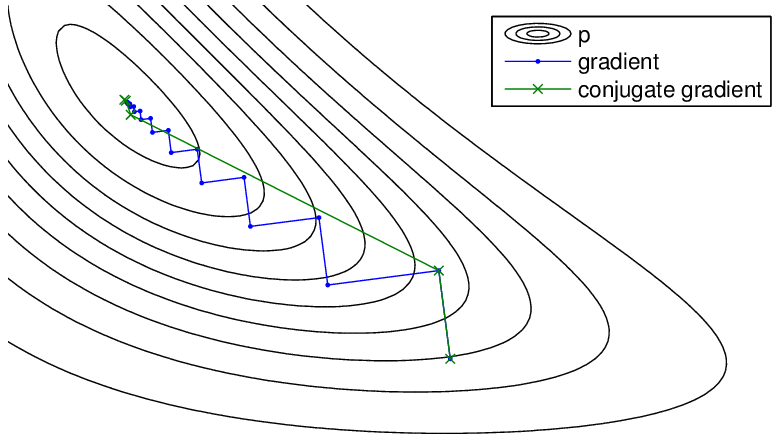
\includegraphics[width=0.5\textwidth]{cg_convergence.png}
  \caption{Conjugate Gradient Method}
  \label{fig:cg}
\end{figure}

\subsection{Arnoldi's method} \label{sec:arnoldi}
The Arnoldi method is a generalization of the Gram-Schmidt orthogonalization process to Krylov subspaces. The Arnoldi method is used to generate an orthonormal basis for the Krylov subspace $\mathcal{K}_m(A, r_0)$.
\begin{algorithm}[H]
  \caption{Arnoldi's method \cite[Algorithm 6.1]{iter_method_saad}}
  \begin{algorithmic}
    \State Choose a vector $v_1$ with $||v_1|| = 1$
    \For{$j = 1, 2, \dots, m$}
    \State $w_j \leftarrow Av_j$
    \For{$i = 1, 2, \dots, j$}
    \State $h_{ij} \leftarrow (w, v_i)$
    \State $w_j \leftarrow w_j - h_{ij}v_i$
    \EndFor
    \State $h_{j+1,j} \leftarrow ||w_j||$
    \State $v_{j+1} \leftarrow w_j / h_{j+1,j}$
    \EndFor
  \end{algorithmic}
  \label{alg:arnoldi}
\end{algorithm}
The Arnoldi method generates an orthonormal basis $V_m = [v_1, v_2, \dots, v_m]$ for the Krylov subspace $\mathcal{K}_m(A, r_0)$ and an upper Hessenberg matrix $\bar{H}_m$ such that
\begin{subequations}\label{eq:arnoldi_decomposition}
  \begin{align}
    AV_m      & = V_m H_m + h_{m+1,m}v_{m+1}e_m^T \label{eqn:arnoldi_decomposition0}, \\
              & = V_{m+1}\bar{H}_m, \label{eqn:arnoldi_decomposition1},               \\
    V^T_mAV_m & = H_m, \label{eqn:arnoldi_decomposition2}
  \end{align}
\end{subequations}
where $e_m$ is the $m$th unit vector and $H_m$ is obtained from $\bar{H}_m$ by removing the last row \cite[Proposition 6.5]{iter_method_saad}.

Note that the Arnoldi method stops at $j$, if and only if the minimal polynomial of $A$ with respect to $v_1$ is of degree $j$ \cite[proposition 6.6]{iter_method_saad}.

\subsection{Arnoldi's method for linear systems}\label{sec:arnoldi_linear_systems}
The Arnoldi method can be used to solve linear systems of the form $Ax = b$. If $v_1 = r_0/||r_0||_2$ and $\beta = ||r_0||_2$, then by \cref{eqn:arnoldi_decomposition2} we have
\[
  V^T_mAV_m = H_m \text{ and } V^T_mr_0 = V^T_m\beta v_1 = \beta e_1 \implies \begin{array}{c}
    H_m y = \beta e_1, \\
    x_m = x_0 + V_m y.
  \end{array} .
\]
This results in the following algorithm
\begin{algorithm}[H]
  \caption{Arnoldi's method for linear systems (FOM) \cite[Algorithm 6.4]{iter_method_saad}}
  \label{alg:arnoldi_linear_systems}
  \begin{algorithmic}
    \State Compute $r_0 = b - Ax_0$, $\beta = ||r_0||_2$ and $v_1 = r_0 / \beta$
    \State Define $H_m = \{0\}$
    \State Define $V_1 = \{v_1\}$
    \For{$j = 1, 2, \dots, m$}
    \State $w_j = Av_j$
    \For{$i = 1, 2, \dots, j$}
    \State $h_{ij} = (w_j, v_i)$ and store $h_{ij}$ in $H_m$
    \State $w_j = w_j - h_{ij}v_i$
    \EndFor
    \State $h_{j+1,j} = ||w_j||_2$
    \If{$h_{j+1,j} = 0$}
    \State $m = j$
    \State break
    \EndIf
    \State $v_{j+1} = w_j / h_{j+1,j}$ and store $v_{j+1}$ into $V_{j+1}$
    \EndFor
    \State Solve $H_m y_m = \beta e_1$ for $y_m$
    \State $x_m = x_0 + V_m y_m$
  \end{algorithmic}
\end{algorithm}

Note that a stopping criterion can be derived from the residual vector $r_m = b - Ax_m$. Theorem \ref{th:arnoldi_residual} gives a way of calculating the size of the residual vector.
\begin{theorem}
  The residual vector $r_m = b - Ax_m$ satisfies
  \begin{subequations}
    \begin{align}
      r_m                                          & = b - Ax_m                                                  \\
                                                   & = r_0 - AV_m y_m                                            \\
      \cref{eqn:arnoldi_decomposition0}\rightarrow & = \beta v_1 - V_m H_m y_m - h_{m+1,m} e_m^T y_m v_{m+1}     \\
                                                   & = - h_{m+1,m} e_m^T y_m v_{m+1}.\label{eq:arnoldi_residual}
    \end{align}
  \end{subequations}
  Therefore, the residual vector is orthogonal to the Krylov subspace $\mathcal{K}_m(A, r_0)$ and its size is given by
  \begin{equation}
    ||r_m||_2 = h_{m+1,m}|e^T_m y_m|,
    \label{eq:arnoldi_residual_size}
  \end{equation}
  where $h_{m+1,m}\geq 0$ \cite[Proposition 6.7]{iter_method_saad}.
  \label{th:arnoldi_residual}
\end{theorem}

\subsection{Lanczos' Algorithm}
In the special case where $A$ is symmetric, the Arnoldi method can be simplified to the Lanczos algorithm. The Lanczos algorithm is a special case of the Arnoldi method where the matrix $T_m = V^T_mAV^T_m$ is tridiagonal given by
\begin{equation}
  T_m =
  \begin{pmatrix}
    \delta_1 & \eta_2   & 0        & \dots  & 0        \\
    \eta_2   & \delta_3 & \eta_3   & \dots  & 0        \\
    0        & \eta_3   & \delta_4 & \dots  & 0        \\
    \vdots   & \vdots   & \vdots   & \ddots & \eta_m   \\
    0        & 0        & 0        & \eta_m & \delta_m
  \end{pmatrix}
  \label{eq:lanczos_tridiagonal}
\end{equation}
This leads to the following algorithm
\begin{algorithm}[H]
  \caption{Lanczos \cite[algorithm 6.15]{iter_method_saad}}
  \begin{algorithmic}
    \State Choose a vector $v_1$ with $||v_1|| = 1$
    \State $\eta_1 = 0$
    \State $v_0 = 0$
    \For{$j = 1, 2, \dots, m$}
    \State $w_j = Av_j - \eta_j v_{j-1}$
    \State $\delta_j = (w_j, v_j)$
    \State $w_j = w_j - \delta_j v_j$
    \State $\eta_{j+1} = ||w_j||$
    \If{$\eta_{j+1} = 0$}
    \State Break
    \EndIf
    \State $v_{j+1} = w_j / \eta_{j+1}$
    \EndFor
  \end{algorithmic}
\end{algorithm}
Similarly, we can apply the Lanczos algorithm to linear systems resulting in \cref{alg:lanczos_linear_systems}.
\begin{algorithm}
  \caption{Lanczos algorithm for linear systems \cite[Algorithm 6.16]{iter_method_saad}}
  \begin{algorithmic}
    \State Compute $r_0 = b - Ax_0$, $\beta = ||r_0||_2$, $v_0 = 0$ and $v_1 = r_0 / \beta$
    \State $V_{1} = \{v_1\}$
    \For{$j = 1, 2, \dots, m$}
    \State $w_j = Av_j - \eta_j v_{j-1}$
    \State $\delta_j = (w_j, v_j)$
    \State $w_j = w_j - \delta_j v_j$
    \State $\eta_{j+1} = ||w_j||_2$
    \If{$\eta_{j+1} = 0$}
    \State $m = j$
    \State Break
    \EndIf
    \State $v_{j+1} = w_j / \eta_{j+1}$ and store $v_{j+1}$ into $V_{j+1}$
    \EndFor
    \State Solve the tridiagonal system $T_m y_m = \beta e_1$ for $y_m$
    \State $x_m = x_0 + V_m y_m$
  \end{algorithmic}
  \label{alg:lanczos_linear_systems}
\end{algorithm}

\subsection{D-Lanczos} The direct version of the Lanczos algorithm or `D-Lanczos' is obtained by performing a LU-factorisation $T_m$
\begin{equation}
  T_m = L_m U_m =
  \begin{pmatrix}
    1              & 0              & 0      & \dots          & 0      \\
    \tilde{\eta}_2 & 1              & 0      & \dots          & 0      \\
    0              & \tilde{\eta}_3 & 1      & \dots          & 0      \\
    \vdots         & \vdots         & \vdots & \ddots         & \vdots \\
    0              & 0              & \dots  & \tilde{\eta}_m & 1
  \end{pmatrix}
  \times
  \begin{pmatrix}
    \tilde{\delta}_1 & \eta_2           & 0                & \dots  & 0                \\
    0                & \tilde{\delta}_2 & \eta_3           & \dots  & 0                \\
    0                & 0                & \tilde{\delta}_3 & \dots  & 0                \\
    \vdots           & \vdots           & \vdots           & \ddots & \eta_m           \\
    0                & 0                & 0                & \dots  & \tilde{\delta}_m
  \end{pmatrix}
  \label{eq:lanczos_lu}
\end{equation}
Then, the approximate solution is given by
\begin{align*}
  x_m & = x_0 + V_m y_m                           \\
      & = x_0 + V_m U_m^{-1} L_m^{-1} \beta e_1   \\
      & = x_0 + V_m U_m^{-1} (L_m^{-1} \beta e_1) \\
      & = x_0 + P_m z_m,
\end{align*}
where $P_m = V_m U_m^{-1}$ and $z_m = L_m^{-1} \beta e_1$. Considering the definition of $U_m$ in \cref{eq:lanczos_lu}, we have that the $m^{\text{th}}$ column of $P_m$ is given by
\begin{equation}
  p_m = \frac{1}{\tilde{\delta}_m}\left[v_m - \eta_m p_{m-1}\right].
  \label{eq:lanczos_p}
\end{equation}
Furthermore, from the LU factorization of $T_m$ we have that
\begin{align*}
  \tilde{\eta}_m   & = \frac{\eta_m}{\tilde{\delta}_{m-1}},       \\
  \tilde{\delta}_m & = \delta_m - \tilde{\eta}_m \eta_m, \ m > 1.
\end{align*}
Now the solution can be incrementally updated by realizing that
\[
  z_m =
  \begin{pmatrix}
    z_{m-1} \\
    \zeta_m
  \end{pmatrix} =
  \begin{pmatrix}
    z_{m-2}     \\
    \zeta_{m-1} \\
    \zeta_m
  \end{pmatrix},
\]
and
\[
  L_m =
  \begin{pmatrix}
    L_{m-1}            & \multicolumn{2}{c}{\mathbf{0}_{m-1}}     \\
    \mathbf{0}_{m-2}^T & \tilde{\eta}_m                       & 1
  \end{pmatrix}.
\]
Then,
\[
  L_m z_m =
  \begin{pmatrix}
    L_{m-1} z_{m-1} \\
    \tilde{\eta}_m \zeta_{m-1} + \zeta_m
  \end{pmatrix} =
  \begin{pmatrix}
    \beta e_1 \\
    0
  \end{pmatrix},
\]
where the last equality follows from definition of $z_m$. Consequently, we have that
\[
  \zeta_m = -\tilde{\eta}_m \zeta_{m-1}.
\]
Finally, we obtain
\begin{align*}
  x_m & = x_0 + P_m z_m                                   \\
      & = x_0 + \left[P_{m-1} \ p_m\right] \begin{pmatrix}
                                             z_{m-1} \\
                                             \zeta_m
                                           \end{pmatrix} \\
      & = x_0 + P_{m-1}z_{m-1} + p_m \zeta_m              \\
      & = x_{m-1} + p_m \zeta_m.
\end{align*}
Putting it all together, we obtain \cref{alg:dlanczos}.
\begin{algorithm}[H]
  \caption{D-Lanczos \cite[Algorithm 6.17]{iter_method_saad}}
  \begin{algorithmic}
    \State $r_0 = b - Ax_0$, $\beta = ||r_0||_2$, $v_1 = r_0 / \beta$
    \State $\tilde{\eta}_1 = \beta_1 = 0$, $p_0 = 0$
    \For{$m = 1, 2, \dots, m$ until convergence}
    \State $w = Av_m - \beta_m v_{m-1}$
    \State $\delta_m = (w, v_m)$
    \If{$m > 1$}
    \State $\tilde{\eta}_m = \frac{\beta_m}{\tilde{\delta}_{m-1}}$
    \State $\zeta_m = -\tilde{\eta}_m \zeta_{m-1}$
    \EndIf
    \State $\tilde{\delta}_m = \delta_m - \tilde{\eta}_m \beta_m$
    \State $p_m = \frac{1}{\tilde{\delta}_m}\left[v_m - \beta_m p_{m-1}\right]$
    \State $x_m = x_{m-1} + p_m \zeta_m$
    \If{convergence criterion is met (using \cref{eq:arnoldi_residual_size} for example)}
    \State break
    \EndIf
    \State $w = w - \delta_m v_m$
    \State $\beta_{m+1} = ||w||_2$
    \State $v_{m+1} = w / \beta_{m+1}$
    \EndFor
  \end{algorithmic}
  \label{alg:dlanczos}
\end{algorithm}
Note that the residual vectors produced by \cref{alg:dlanczos} are orthogonal to each other due to \cref{th:arnoldi_residual}. Additionally,
\begin{align*}
  P^T_m A P_m & = U_m^{-T} V_m^T A V_m U_m^{-1} \\
              & = U_m^{-T} T_m U_m^{-1}         \\
              & = U_m^{-T} L_m,
\end{align*}
where $U_m^{-T}$ and $L_m$ are both lower diagonal matrices. Their product must be symmetric, since $P^T_m A P_m$ is (symmetry of $A$). Therefore, $U_m^{-T} L_m$ must be a diagonal matrix. Consequently, the vectors $p_m$ are $A$-orthogonal to each other.

\subsection{Derivation of CG}
From observations made in the in \cref{alg:dlanczos}, we can derive the conjugate gradient method. We start by constraining subsequent residuals $r_j$ to be orthogonal and search directions $p_j$ to be $A$-orthogonal to each other. To that end, let
\begin{equation}
  x_{j+1} = x_j + \alpha_j p_j,
  \label{eq:cg_solution_update}
\end{equation}
and, thereby,
\begin{equation}
  r_{j+1} = r_j - \alpha_j A p_j.
  \label{eq:cg_residual_update}
\end{equation}
If the residuals are to be orthogonal, then
\[
  (r_{j+1}, r_j) = 0 \implies (r_j - \alpha_j A p_j, r_j) = 0 \implies \alpha_j = \frac{(r_j, r_j)}{(A p_j, r_j)}.
\]
Now, using \cref{eq:lanczos_p,eq:arnoldi_residual}, we can write the next search direction as a linear combination of the previous search direction and the next residual
\begin{equation}
  p_{j+1} = r_{j+1} + \beta_j p_j.
  \label{eq:cg_search_direction_update}
\end{equation}
Substituting \cref{eq:cg_search_direction_update}, we obtain
\[
  (Ap_{j+1}, r_j) = (Ap_j, p_j -\beta_{j-1}p_{j_1}) = (Ap_j, p_j),
\]
since $p_j$ is $A$-orthogonal to $p_{j-1}$. This allows us to write
\begin{equation}
  \alpha_j = \frac{(r_j, r_j)}{(A p_j, p_j)}.
  \label{eq:cg_alpha}
\end{equation}
Additionally, taking the inner product with $A p_j$ on both sides of \cref{eq:cg_search_direction_update} gives
\[
  \beta_j = \frac{(r_{j+1}, A p_j)}{(p_j, A p_j)}.
\]
Now, rewriting \cref{eq:cg_residual_update} gives
\[
  Ap_j = \frac{1}{\alpha_j} (r_j - r_{j+1}),
\]
which we substitute into the equation for $\beta_j$ to obtain
\begin{equation}
  \beta_j = \frac{1}{\alpha_j}\frac{(r_{j+1}, (r_{j+1}-r_j))}{(Ap_j, r_j)} = \frac{(r_{j+1},r_{j+1})}{((r_j - r_{j-1}), r_j)} = \frac{(r_{j+1},r_{j+1})}{(r_j, r_j)}.
  \label{eq:cg_beta}
\end{equation}
Finally, we can write the conjugate gradient method as \cref{alg:cg}.
\begin{algorithm}[H]
  \caption{Conjugate Gradient Method \cite[Algorithm 6.18]{iter_method_saad}}
  \begin{algorithmic}
    \State $r_0 = b - Ax_0$, $p_0 = r_0$, $\beta_0 = 0$
    \For{$j = 0, 1, 2, \dots, m$}
    \State $\alpha_j = (r_j, r_j) / (A p_j, p_j)$
    \State $x_{j+1} = x_j + \alpha_j p_j$
    \State $r_{j+1} = r_j - \alpha_j A p_j$
    \State $\beta_j = (r_{j+1}, r_{j+1}) / (r_j, r_j)$
    \State $p_{j+1} = r_{j+1} + \beta_j p_j$
    \EndFor
  \end{algorithmic}
  \label{alg:cg}
\end{algorithm}

\paragraph{Hessenberg matrix coefficients} The coefficients of the Hessenberg matrix $T_m$ can be calculated as follows
\begin{equation}
  \delta_{j+1} =
  \begin{cases}
    \frac{1}{\alpha_j} + \frac{\beta_{j-1}}{\alpha_{j-1}} & j > 0, \\
    \frac{1}{\alpha_0}                                    & j = 0,
  \end{cases}
  \label{eq:cg_hessenberg_delta}
\end{equation}
and
\begin{equation}
  \eta_{j+1} = \frac{\sqrt{\beta_{j-1}}}{\alpha_{j-1}}.
  \label{eq:cg_hessenberg_eta}
\end{equation}
here we have used the definition of $T_m = V_m^T A V_m$ and the fact that the residuals are just multiples of the Lanczos vectors $r_j = \text{scalar} \times v_j$ by \cref{eq:arnoldi_residual} \cite[Equation 6.103]{iter_method_saad}.

\subsection{Convergence of CG}
\subsubsection{Convergence rate}\label{sec:cg_convergence_rate}
It can be shown \cite[lemma 6.28 and theorem 6.29]{iter_method_saad} that the error of the $m^{\text{th}}$ iterate of the CG algorithm $\epsilon_m = x^* - x_m$ minimizes the $A$-norm of the error in the affine Krylov subspace $\mathcal{K}_m(A, r_0)$, that is
\[
  ||(I - Aq_m(A))\epsilon_0||_A = \min_{q \in \mathcal{P}_{m-1}} ||(I - Aq(A))\epsilon_0||_A = \min_{r \in \mathcal{P}_{m-1}, r(0) = 1} ||r(A)\epsilon_0||_A,
\]
where the equality follows, since there exists an isomorphic mapping between the affine Krylov subspace and the polynomial space $\mathcal{P}_{m-1}$ of degree $m-1$ and the polynomial $tq(t)$ equals $0$ at $t=0$. The right-hand side can be further bounded by letting $\lambda_i, \xi_i$ be the eigenvalues of $A$ and the components of $\epsilon_0$ in the eigenvector basis of $A$, respectively. Then
\[
  ||r(A)\epsilon_0||_A = \sqrt{\sum_{i=1}^n |r(\lambda_i)|^2 |\xi_i|^2} \leq \max_{\lambda \in \sigma(A)} |r(\lambda)| ||\epsilon_0||_A,
\]
where $\sigma(A)$ is the spectrum of $A$. This gives
\begin{align*}
  ||e_m||                                                                                                                            & \leq \min_{r \in \mathcal{P}_{m-1}, r(0) = 1} \max_{\lambda \in \sigma(A)} |r(\lambda)| ||\epsilon_0||_A \\
  \text{Chebyshev polynomial } C_m \text{, } \eta=\frac{\lambda_{\text{min}}}{\lambda_{\text{max}}-\lambda_{\text{min}}} \rightarrow & \frac{||\epsilon_0||_A}{C_m(1+2\eta)}                                                                    \\
                                                                                                                                     & \leq \frac{2||\epsilon_0||_A}{\left(1 + 2\eta + 2\sqrt{\eta(\eta+1)}\right)^m}                           \\
                                                                                                                                     & = \frac{2||\epsilon_0||_A}{\left(\sqrt{\eta} + \sqrt{\eta + 1}\right)^{2m}}                              \\
                                                                                                                                     & = 2 \left(\frac{\sqrt{\kappa}-1}{\sqrt{\kappa} + 1}\right)^m ||\epsilon_0||_A,
\end{align*}
where $\kappa = \lambda_{\text{max}}/\lambda_{\text{min}}$ is the condition number of (symmetric matrix) $A$. To sum up
\begin{theorem}
  The error of the $m^{\text{th}}$ iterate of the CG algorithm is bounded by
  \begin{equation}
    ||e_m|| \leq 2 \left(\frac{\sqrt{\kappa}-1}{\sqrt{\kappa} + 1}\right)^m ||\epsilon_0||_A,
    \label{eq:cg_convergence_rate}
  \end{equation}
  where $\kappa = \lambda_{\text{max}}/\lambda_{\text{min}}$ is the condition number of (symmetric matrix) $A$.
  \label{th:cg_convergence_rate}
\end{theorem}
During the derivation of \cref{th:cg_convergence_rate}, we obtain the general expression for the error of the $m^{\text{th}}$ iterate of the CG algorithm
\[
  || e_m|| \leq \min_{r \in \mathcal{P}_{m}, r(0) = 1} \max_{\lambda \in \sigma(A)} |r(\lambda)| ||\epsilon_0||_A \\
\]
Now define,
\[
  r_{\textrm{test}}(t) = \prod_{i=1}^m \frac{\lambda_i - t}{\lambda_i}.
\]
Note that $r_{\textrm{test}}\in\mathcal{P}_m$, since it has degree $m$. Also, $r_{\textrm{test}}(0) = 1$ and $r_{\textrm{test}}(\lambda_i) = 0$ for $i = 1, 2, \dots, m$. Hence, $r_{\textrm{test}}$ is a polynomial that satisfies the constraints of the minimization problem. We obtain for $m = N$ that
\[
  ||e_N||_A = ||\epsilon_0||_A \max_{\lambda \in \sigma(A)} |r_{\textrm{test}}(\lambda)| = 0,
\]
which implies that CG converges in $N$ iterations in exact arithmetic. Furthermore, if there are only $k$ distinct eigenvalues, then the CG iteration terminates in at most $k$ iterations.

\subsubsection{Condition number estimation} \label{sec:cg_condition_number_estimate}
During CG iterations it is possible to get an estimate of the condition number of the matrix $A$ by using the tridiagonal Hessenberg matrix $T_m$ and the recurrence relation for determinant of tridiagonal matrices. Suppose the characteristic polynomial of $T_j$ is given by $p_{T_j}(\lambda)$, then
\begin{align*}
  p_{T_0}(\lambda) & = 1,                                                                   \\
  p_{T_1}(\lambda) & = \lambda - \delta_1,                                                  \\
  p_{T_2}(\lambda) & = (\lambda - \delta_2)p_{T_1}(\lambda) - \eta_2^2,                     \\
  p_{T_3}(\lambda) & = (\lambda - \delta_3)p_{T_2}(\lambda) - \eta_3^2(\lambda - \delta_1), \\
                   & \vdots                                                                 \\
\end{align*}
Hence, the characteristic polynomial of $T_j$ can be written as
\begin{align}
  p_{T_j}(\lambda) & = (\lambda - \delta_j)p_{T_{j-1}}(\lambda) - \eta_j^2p_{T_{j-2}}
  \label{eq:cg_hessenberg_char_poly}.
\end{align}
Now the condition number of $A$ is defined as
\[
  \kappa(A) = ||A||_2 ||A^{-1}||_2 = \max_{x\in\mathbb{R}^n, x\neq0} \frac{||Ax||_2}{||x||_2} \max_{x\in\mathbb{R}^n, x\neq0} \frac{||A^{-1}x||_2}{||x||_2}.
\]
Similarly, the condition number of $T_j$ is defined as
\[
  \kappa(T_j) = ||T_j||_2 ||T_j^{-1}||_2 = \max_{x\in\mathbb{R}^j, x\neq0} \frac{||T_jx||_2}{||x||_2} \max_{x\in\mathbb{R}^j, x\neq0} \frac{||T_j^{-1}x||_2}{||x||_2}.
\]
Note that
\begin{align*}
  \max_{x\in\mathbb{R}^j, x\neq0} \frac{||T_jx||_2}{||x||_2} & = \max_{x\in\mathbb{R}^n, x\neq0} \frac{||V_j^T A V_j x||_2}{||x||_2}                        \\
  \text{orthogonality of } V_j \rightarrow                   & = \max_{x\in\mathbb{R}^n, x\neq0} \frac{||V_j(V_j^T A V_j x)||_2}{||V_j x||_2}               \\
                                                             & = \max_{x\in\mathbb{R}^j, x\neq0} \frac{||A V_j x||_2}{||V_j x||_2}                          \\
                                                             & = \max_{\tilde{x}\in\mathcal{K}_j, \tilde{x}\neq0} \frac{||A \tilde{x}||_2}{||\tilde{x}||_2} \\
                                                             & \approx ||A||_2,
\end{align*}
and similarly for the inverse. Presumably, the estimate will get better as $j$ increases and the Krylov subspace $\mathcal{K}_j$ gets closer to the eigenspace of $A$. \todo{Find proof of this}.

Now, combining this with the recurrence relation for the characteristic polynomial of $T_j$ in \cref{eq:cg_hessenberg_char_poly}, we have a way of estimating the condition number of $A$. In particular, at any iteration $j$ of the CG algorithm, let $\tilde{\lambda}_{\text{max}}$ and $\tilde{\lambda}_{\text{min}}$ be the maximum and minimum zeroes of $p_{T_j}$. Then, the condition number of $A$ is approximately given by
\begin{equation}
  \kappa(A) \approx \frac{\tilde{\lambda}_{\text{max}}}{\tilde{\lambda}_{\text{min}}}.
  \label{eq:cg_condition_number_estimate}
\end{equation}

\subsubsection{Influence of eigenvalue distribution on convergence}\label{sec:cg_eigenvalue_distribution}
In the derivation of the convergence rate of the CG algorithm in \ref{th:cg_convergence_rate}, we used the Chebyshev polynomial to bound the error. However, we can find an expression of the error provided the eigendecomposition of $A$ is available. Suppose $A = VDV^T$, then $r(A) = I - Aq(A) = V(I - Dq(D))V^T = Vr(D)V^T$. Also note that $e_0 = x^* - x_0 = A^{-1}b - x_0 = A^{-1}r_0$. As seen in \cref{sec:cg_convergence_rate}, the error of the $m^{\text{th}}$ iterate of the CG algorithm is given by
\begin{equation*}
  ||e_m||_A^2 = ||r_m(A)\epsilon_0||_A^2,
\end{equation*}
and
\begin{align*}
  ||r_m(A)\epsilon_0||_A^2 & = \epsilon_0^T r_m(A)^T A r_m(A) \epsilon_0                 \\
                           & = \epsilon_0^T V r_m(D) V^T V D V^T V r_m(D) V^T \epsilon_0 \\
                           & = (V^T\epsilon_0)^T r_m(D) D r_m(D) V^T \epsilon_0.
\end{align*}
We also have
\begin{align*}
  V^T\epsilon_0 & = V^T A^{-1} r_0       \\
                & = V^T V D^{-1} V^T r_0 \\
                & = D^{-1} \rho_0,
\end{align*}
where $\rho_0 = V^T r_0$ is the initial residual in the eigenvector basis of $A$. Therefore,
\begin{align*}
  ||r_m(A)\epsilon_0||_A^2 & = \rho_0^T D^{-1} r_m(D) D r_m(D) D^{-1} \rho_0                 \\
                           & = \rho_0^T r_m(D) D^{-1} r_m(D)  \rho_0                         \\
                           & = \sum_{i=1}^n \frac{r_m(\lambda_i)^2}{\lambda_i} \rho_{0,i}^2,
\end{align*}
which gives
\begin{equation}
  ||e_m||_A^2 = \sum_{i=1}^n \frac{r_m(\lambda_i)^2}{\lambda_i} \rho_{0,i}^2.
  \label{eq:cg_error_eigenvalue}
\end{equation}

To obtain the residual polynomial $r_m$, we can use the recurrence relation between the Lanczos vectors and expressions for the Hessenberg matrix coefficients in \cref{eq:cg_hessenberg_delta,eq:cg_hessenberg_eta}. In particular,
\begin{align*}
  \frac{1}{\eta_{j+1}} v_j & = A v_j - \delta_j v_j - \eta_j v_{j-1} \\
                           & = p_{j+1}(A) v_1,
\end{align*}
where we define $p_{-1}(A) = 0, p_0(A) = I$. This gives
\begin{align*}
  \eta_{j+1}p_{j+1}(A)v_1 & = A v_j - \delta_j v_j - \eta_j v_{j-1},                            \\
                          & = \left( A p_j(A) - \delta_j p_j(A) - \eta_j p_{j-1}(A) \right)v_1, \\
\end{align*}
and therefore
\begin{equation}
  p_{j+1}(A) = \frac{1}{\eta_{j+1}}\left( (A - \delta_j )p_j(A) - \eta_j p_{j}(A) \right).
  \label{eq:cg_lanczos_polynomial}
\end{equation}
Furthermore, we have the following relation between the residual polynomial and the Lanczos polynomial \cite[Section 3.2]{Meurant_Strakoš_2006}
\begin{equation}
  r_{j}(A) = (I-Aq_{j-1}(A))r_0 = \frac{p_{j}(A)}{p_{j}(0)}r_0.
  \label{eq:cg_residual_polynomial}
\end{equation}
This gives a way of calculating the residual polynomial $r_m$ and thereby the error of the $m^{\text{th}}$ iterate of the CG algorithm.

Additionally, the coefficients $c_i$ of the solution polynomial $q_m$ in \cref{eq:cg_approximate_solution} can be calculated. First we introduce a function that extracts the coefficients of a polynomial $p$
\begin{definition}
  Let $p(t) = \sum_{i=0}^n c_i t^i$ be a polynomial of degree $n$. Then, the function $\text{coeff}(p;i)$ extracts the $i^{\text{th}}$ coefficient of $p$ such that $\text{coeff}(p;i) = c_i$.
\end{definition}
Now using \cref{eq:cg_residual_polynomial}, we can write the solution polynomial as
\begin{align*}
                              & Aq_{m-1}(A) = I - r_m(A)                                                  \\
  r_m(\mathbf{0}) = I\implies & A\sum_{i=1}^{m-1} c_{i-1} A^i = -\sum_{i=1}^{m} \text{coeff}(r_m; i) A^i,
\end{align*}
which implies
\begin{equation}
  c_i = -\text{coeff}(r_m; i+1), \quad i = 0, 1, \dots, m-1.
  \label{eq:cg_solution_coefficients}
\end{equation}
\begin{figure}[H]
  \centering
  \includegraphics[width=\textwidth]{cg_convergence_behaviour.pdf}
  \caption{Residual polynomials resulting from successive CG iterations}
  \label{fig:cg_convergence_behaviour}
\end{figure}

The behavior of the residual polynomials is crucial for understanding the convergence properties of the CG method. In particular, the distribution of the eigenvalues of $A$ significantly affects the convergence rate, as illustrated in \cref{fig:cg_effect_of_eigenvalue_distribution}.
\begin{figure}[H]
  \centering
  \includegraphics[width=\textwidth]{effect_of_eigenvalue_distribution.pdf}
  \caption{Plots of the last three CG residual polynomials for different eigenvalue distributions. $n_c$ indicates  the number of clusters and $\sigma$ is the width of the cluster. The size of the system $n$ and the condition number $\kappa(A)$ are kept constant.}
  \label{fig:cg_effect_of_eigenvalue_distribution}
\end{figure}
Hence, the number of iterations required for convergence depends on the specific clustering of the eigenvalues, as pointed out for example in \citeauthor[Section 2.3]{nonlinear_cg_Kelley_1995}.

From the behavior exhibited in figure \cref{fig:cg_effect_of_eigenvalue_distribution} as well as from \cref{th:cg_krylov_dimension} we can reason what the best and worst possible spectra for CG convergence are. That is, the best possible spectrum is one where eigenvalues are tightly clustered around distinct values, while the worst possible spectrum is one where the eigenvalues are evenly distributed across the whole range of the spectrum. This is illustrated in \cref{fig:cg_best_worst_spectra}.
\begin{figure}[H]
  \centering
  \includegraphics[width=\textwidth]{cg_convergence_extreme_spectra.pdf}
  \caption{Best and worst possible spectra for CG convergence}
  \label{fig:cg_best_worst_spectra}
\end{figure}

\subsection{Preconditioning} \label{sec:cg_preconditioning}
Suppose $M$ is some SPD preconditioner, then variants of CG can be derived by applying $M$ to the system of equations. The three main approaches are
\begin{enumerate}[label=\roman*,ref=preconditioner-type \roman*]
  \item\label{pcg_type:left} left
  \begin{align*}
    M^{-1}Ax & = M^{-1}b
  \end{align*}
  \item\label{pcg_type:right} right
  \begin{align*}
    AM^{-1}u & = M^{-1}b  \\
    x        & = M^{-1}u;
  \end{align*}
  \item\label{pcg_type:symmetric} symmetric or split
  \begin{align*}
    M              & = LL^T     \\
    x              & = L^{-T}u  \\
    L^{-1}AL^{-T}u & = L^{-1}b.
  \end{align*}
\end{enumerate}
Furthermore, all these variants are mathematically equivalent in some sense. Indeed, for the cases \cref{pcg_type:left} and \cref{pcg_type:right}, we can rewrite the CG algorithm using the $M-$ or $M^{-1}-$inner products, respectively. In either case the iterates are the same. For instance for the left preconditioned CG, we define $z_j = M^{-1}r_j$. Note that $M^{-1}A$ is self-adjoint with respect to the $M-$inner product, that is
\[
  (M^{-1}Ax, y)_M = (Ax, y) = (x, Ay) = (x, M^{-1}Ay)_M.
\]
We use this to get a new expression for $\alpha_j$. To that end, we write
\begin{align*}
  0 & = (r_{j+1}, r_j)_M                                        \\
    & = (z_{j+1}, r_j)                                          \\
    & = (z_j - \alpha_j M^{-1}Ap_j, M^{-1}r_j)_M                \\
    & = (z_j, M^{-1}r_j)_M - \alpha_j (M^{-1}Ap_j, M^{-1}r_j)_M \\
    & = (z_j, z_j)_M - \alpha_j (M^{-1}Ap_j, z_j)_M             \\
\end{align*}
and therefore
\[
  \alpha_j = \frac{(z_j, z_j)_M}{(M^{-1}Ap_j, z_j)_M}.
\]
Using $p_{j+1} = z_{j+1} + \beta_j p_j$ and A-orthogonality of the search directions with respect to $M-$norm $(Ap_j, p_k)_M = 0$ (), we can write
\[
  \alpha_j = \frac{(z_j, z_j)_M}{(M^{-1}Ap_j, p_j)_M}.
\]
Similarly, we can derive the equivalent expression of \cref{eq:cg_beta} as
\[
  \beta_j = \frac{(z_{j+1}, z_{j+1})_M}{(z_j, z_j)_M}.
\]
This gives the left preconditioned CG algorithm in \cref{alg:pcg_left}.
\begin{algorithm}[H]
  \caption{Left preconditioned CG \cite[Algorithm 9.1]{iter_method_saad}}
  \label{alg:pcg_left}
  \begin{algorithmic}
    \State $r_0 = b - Ax_0$, $z_0 = M^{-1}r_0$, $p_0 = z_0$, $\beta_0 = 0$
    \For{$j = 0, 1, 2, \dots, m$}
    \State $\alpha_j = (z_j, z_j)_M / (M^{-1}Ap_j, p_j)_M = (r_j, z_j) / (Ap_j, p_j)$
    \State $x_{j+1} = x_j + \alpha_j p_j$
    \State $r_{j+1} = r_j - \alpha_j A p_j$
    \State $z_{j+1} = M^{-1}r_{j+1}$
    \State $\beta_j = (z_{j+1}, z_{j+1})_M / (z_j, z_j)_M = (r_{j+1}, z_{j+1}) / (r_j, z_j)$
    \State $p_{j+1} = z_{j+1} + \beta_j p_j$
    \EndFor
  \end{algorithmic}
\end{algorithm}
Furthermore it can be shown that the iterates of CG applied to the system with \cref{pcg_type:symmetric} results in identical iterates \cite[Algorithm 9.2]{iter_method_saad}.

\subsubsection{Examples of preconditioners} \label{sec:cg_preconditioners}
\paragraph{$q(A)$ polynomial preconditioner}
If the spectrum of $A$ is approximately known, and we have a way of approximating the solution polynomial from \cref{eq:cg_solution_coefficients}, then we can use this polynomial as a preconditioner. This is known as the $q(A)$ polynomial preconditioner. That is
\begin{align*}
  M^{-1} = q(A), \\
  M^{-1}A = M^{-1}b.
\end{align*}
\newpage
\section{Generalized Minimal Residual Method}\label{sec:gmres}
This section is largely based on Section 6.5 from the book by \citeauthor{iter_method_saad} about iterative methods.

CG is limited to symmetric positive definite matrices, but the Generalized Minimal Residual Method (GMRES) can be used for general matrices.

GMRES is a Krylov subspace projection method with $\mathcal{K} = \mathcal{K}_m$ and $\mathcal{L} = A\mathcal{K}_m$. This method minimizes the residual norm, as is described in \cref{sec:projm_projectors} with \cref{eq:projm_residual_projection} and later in \cref{sec:cg_variants} with the second instance of \cref{cg_type:direct}.

Furthermore, GMRES is similar to Arnoldi's method for linear systems (see \cref{sec:arnoldi,sec:arnoldi_linear_systems}). The only difference being that instead of performing a system solve after determining the Hessenberg matrix $H_m$, GMRES performs a least squares solve to find vector that minimizes the residual norm. To show this note that $x_m = x_0 + V_m y$ and consider
\begin{align*}
    b - Ax_m                                               & = b - A(x_0  + V_my)               \\
                                                           & = r_0 - AV_my                      \\
    \textrm{\cref{eqn:arnoldi_decomposition1}} \rightarrow & = \beta v_1 - V_{m+1}\bar{H}_m y   \\
                                                           & = V_{m+1}(\beta e_1 - \bar{H}_m y) \\
\end{align*}
Now, using orthonormality of $V_{m+1}$, we can write
\begin{align*}
    y & = \underset{y}{\text{argmin}} ||b - Ax_m||                        \\
      & = \underset{y}{\text{argmin}}||V_{m+1}(\beta e_1 - \bar{H}_m y)|| \\
      & = \underset{y}{\text{argmin}} ||\beta e_1 - \bar{H}_m y||,        \\
\end{align*}
which is a least squares problem.

Even though GMRES is the same as \cref{alg:arnoldi_linear_systems} with a least squares solve instead of a system solve, the algorithm is presented in \cref{alg:gmres} for completeness.
\begin{algorithm}[H]
    \caption{GMRES \cite[Algorithm 6.9]{iter_method_saad}}
    \label{alg:gmres}
    \begin{algorithmic}[1]
        \State Compute $r_0 = b - Ax_0$, $\beta = ||r_0||_2$ and $v_1 = r_0 / \beta$
        \State Define $H_m = \{0\}$
        \State Define $V_1 = \{v_1\}$
        \For{$j = 1, 2, \dots, m$}
        \State $w_j = Av_j$
        \For{$i = 1, 2, \dots, j$}
        \State $h_{ij} = (w_j, v_i)$ and store $h_{ij}$ in $H_m$
        \State $w_j = w_j - h_{ij}v_i$
        \EndFor
        \State $h_{j+1,j} = ||w_j||_2$
        \If{$h_{j+1,j} = 0$}
        \State $m = j$
        \State break
        \EndIf
        \State $v_{j+1} = w_j / h_{j+1,j}$ and store $v_{j+1}$ into $V_{j+1}$
        \EndFor
        \State Construct Hessenberg matrix $\bar{H}_m \in \mathbb{R}^{(m+1)\times m}$
        \State Solve the least squares problem $\min_{y \in \mathbb{R}^m} ||\beta e_1 - \bar{H}_m y||_2$
        \State $x_m = x_0 + V_m y_m$
    \end{algorithmic}
\end{algorithm}

\subsection{GMRES implementation details}
Algorithm \ref{alg:gmres} does not explicitly produce successive approximations $x_k$ as in \cref{alg:arnoldi_linear_systems}. Hence, it is cumbersome to check for convergence. Moreover, employing a monolithic least squares solve at the end of the algorithm does not allow the use of intermediary results like in \cref{alg:arnoldi_linear_systems} or \cref{alg:dlanczos}.

To tackle these issues, one can apply a rotation to the Hessenberg matrix at each iteration in order to make it upper triangular. The $i^{\textrm{th}}$ rotation matrix is of the form \cite[Equation 6.34]{iter_method_saad}
\begin{equation}
    \Omega_i =
    \begin{pmatrix}
        1 &        &   &      &  &     &   &        &   \\
          & \ddots &   &      &  &     &   &        &   \\
          &        & 1 &      &  &     &   &        &   \\
          &        &   & c_i  &  & s_i &   &        &   \\
          &        &   & -s_i &  & c_i &   &        &   \\
          &        &   &      &  &     & 1 &        &   \\
          &        &   &      &  &     &   & \ddots &   \\
          &        &   &      &  &     &   &        & 1 \\
    \end{pmatrix},
\end{equation}
where \cite[Equation 6.37]{iter_method_saad}
\begin{align*}
    c_i & = \frac{h^(i-1)_{ii}}{\sqrt{h^(i-1)_{ii}^2 + h_{i+1,i}^2}}, \\
    s_i & = \frac{h_{i+1,i}}{\sqrt{h^(i-1)_{ii}^2 + h_{i+1,i}^2}},
\end{align*}
and $h^(i-1)_ii$ is the $i^{\textrm{th}}$ diagonal element of the Hessenberg matrix after $i-1$ iterations and rotations $\bar{H}^(i-1)_{i-1}$. That is 
\[
    \bar{H}^(k)_k = \Omega_{k}\dots\Omega_1\bar{H}_k = Q_k\bar{H}_k,
\]
where
\[
    Q_k = \Omega_k\dots\Omega_1.
\]
Define 
\begin{subequations}
    \begin{align}
        \bar{R}_k &= \bar{H}^(k)_k \label{eq:gmres_Rk}, \\
        \bar{g}_k &= Q_k(\beta e_1) = (\gamma_1, \dots, \gamma_{k+1})^T \label{eq:gmres_gk}.
    \end{align}
\end{subequations} Note that 
\[
    \det(\Omega_i) = 1, \quad \forall i,
\]
and, therefore, $\det(Q_k) = 1$. This implies that $Q_k$ is unitary. Consequently,
\[
    \min\|\beta e_1 - \bar{H}_m y\| = \min\|Q_m(\beta e_1 - \bar{H}_m y)\| = \min\|\bar{g}_m - \bar{R}_m y\|.
\]
The following theorem is then obtained \cite[Proposition 6.9]{iter_method_saad}.
\begin{theorem}
    Let $m \leq n$ and $\Omega_i, i=1, \ldots, m$ be the rotation matrices used to transform $\bar{H}_m$ into an upper triangular form. Denote by $\bar{R}_m, \bar{g}_m=\left(\gamma_1, \ldots, \gamma_{m+1}\right)^T$ the resulting matrix and right-hand side, as defined by \cref{eq:gmres_Rk,eq:gmres_gk} and by $R_m, g_m$ the $m \times m$ upper triangular matrix and m-dimensional vector obtained from $\bar{R}_m, \bar{g}_m$ by deleting their last row and component respectively. Then,
    \begin{enumerate} [label=\roman*, ref=rotated GMRES\roman*]
        \item\label{rotated_gmres:rank} The rank of $AV_m$ is equal to the rank of $R_m$. In particular, if $r_{m m} = 0$ then $A$ must be singular.
        \item\label{rotated_gmres:least_squares} The vector $y_m$ which minimizes $\|\beta e_1 - \bar{H}_m y\|_2$ is given by
              \[
                  y_m = R_m^{-1} g_m.
              \]
        \item\label{rotated_gmres:residual} The residual vector at step $m$ satisfies 
              \[
                  b - Ax_m = V_{m+1}(\beta e_1 - \bar{H}_m y_m) = V_{m+1}Q_m^T(\gamma_{m+1}e_{m+1}),
              \]
              and, as a result,
              \[
                  \|b - Ax_m\|_2 = |\gamma_{m+1}|.
              \]
    \end{enumerate}
\end{theorem}

Item \ref{rotated_gmres:residual} is particularly useful for checking convergence, as \cite[Equation 6.47]{iter_method_saad}
\[
    \gamma_{k+1} = -s_j\gamma_j.
\]
Therefore, 
\begin{equation}
    \|r_k\| = |s_k||\gamma_k|.
    \label{eq:gmres_residual}
\end{equation}

\subsection{Relation between GMRES and CG}
\todo{Talk about how the iterates of the (rotated) GMRES method are related to the iterates of the CG method.}
\newpage
\section{Nonlinear systems}\label{sec:nonlinear_systems}
We start out with a general formulation of a nonlinear system of equations. Define the non-linear operator $F: \mathbb{R}^N\rightarrow \mathbb{R}^N$ as
\begin{equation}
  F(x) = 0,
  \label{eq:nonlinear_system}
\end{equation}
Some general restrictions are placed on $F$, which can be weakened depending on the method
\begin{enumerate}[label=\roman*,ref=$F$-criterium \roman*]
  \item\label{F_criteria:existence} Existence: \ref{eq:nonlinear_system} has a solution $x^*$.
  \item\label{F_criteria:lipschitz} Lipschitz continuity: $F': \Omega \rightarrow \mathbb{R}^{N \times N}$ is Lipschitz continuous with constant $\gamma$.
  \item\label{F_criteria:nonsigular} Non-singularity: $F'(x^*)$ is nonsingular.
\end{enumerate}
Define $\mathbb{B}(r) = \{x\in\mathbb{R}^N| ||e||<r\}$ to be the ball of radius $r$ centered at the one of the roots of $F$ with $e = x-x^{*}$. The following theorem then follows from the restrictions above \cite[lemma 4.3.1]{nonlinear_cg_Kelley_1995}.
\begin{theorem}
  Assume that the standard assumptions \cref{F_criteria:existence,F_criteria:lipschitz,F_criteria:nonsigular} hold. Then there is $\delta>0$ so that for all $x \in \mathcal{B}(\delta)$
  \begin{align}
    \left\|F^{\prime}(x)\right\|      & \leq 2\left\|F^{\prime}\left(x^*\right)\right\|      \\
    \left\|F^{\prime}(x)^{-1}\right\| & \leq 2\left\|F^{\prime}\left(x^*\right)^{-1}\right\|
  \end{align}
  and
  \begin{equation}
    \frac{\|e\|}{2\left\|F^{\prime}\left(x^*\right)^{-1}\right\|}  \leq\|F(x)\| \leq 2\left\|F^{\prime}\left(x^*\right)\right\|\|e\|
  \end{equation}
  \label{thm:nonlinear_system}
\end{theorem}

Various kinds of convergence known as `q-type' for iteration techniques can be defined for nonlinear systems. The following definitions are taken from \cite[Section 4.3]{nonlinear_cg_Kelley_1995}. If $x_k \rightarrow x^{*}$, then for $k$ sufficiently large, there exists convergence that is:
\begin{enumerate}[label=\roman*,ref=nonlinear \roman*]
  \item\label{conv_type:qlinear} q-linear with q-factor $\nu \in(0,1)$
  \[
    ||x_{k+1} - x^*|| \leq \nu ||x_k - x^*||,
  \]
  \item\label{conv_type:qsuper_linear} q-superlinear
  \[
    \lim_{k\rightarrow\infty} \frac{||x_{k+1} - x^*||}{||x_k - x^*||} = 0,
  \]
  \item\label{conv_type:qquadratic} q-quadratic with constant $C>0$
  \[
    ||x_{k+1} - x^*|| \leq C ||x_k - x^*||^2,
  \]
  \item\label{conv_type:qsuper_linear_order} q-quadratic with q-order $\mu > 1$ and constant $C>0$
  \[
    ||x_{k+1} - x^*|| \leq C ||x_k - x^*||^{\mu}.
  \]
\end{enumerate}
For instance, Fixed Point (FP) or Richardson iteration method is q-linear with constant equal to the Lipschitz constant of the operator \cite[Theorem 4.2.1]{nonlinear_cg_Kelley_1995}. Moreover, assuming \cref{F_criteria:existence,F_criteria:lipschitz,F_criteria:nonsigular} hold, then Newton's method is q-quadratic with $C = \gamma \|F'(x^*)\|$ provided that the initial guess is close enough to the solution \cite[Theorem 5.1.2]{nonlinear_cg_Kelley_1995}. Additionally, The chord method is q-linear with q-factor $\nu = C_C\|e_0\|$ \cite[Theorem 5.4.2]{nonlinear_cg_Kelley_1995}, where $C_C = \bar{C}(1+2\gamma)$ and $\bar{C} = C + 16 \|F(x^*)^{-1}\|^2\|F(x^*)\| + 4\|F(x^*)^{-1}\|$ \cite[Theorem 5.4.1]{nonlinear_cg_Kelley_1995}.

Moreover, it can occur that the operator $F$ introduces errors that are independent of the approximation error. In this case a different kind of convergence `r-type' is used to describe the behavior of the method \cite[Definition 4.1.3]{nonlinear_cg_Kelley_1995}
\begin{definition}
  Let $\left\{x_n\right\} \subset R^N$ and $x^* \in R^N$. Then $\left\{x_n\right\}$ converges to $x^*$ r-(quadratically, super-linearly, linearly) if there is a sequence $\left\{\xi_n\right\} \subset R$ converging q-(quadratically, super-linearly, linearly) to zero such that
  \[
    \left\|x_n-x^*\right\| \leq \xi_n
  \]
  We say that $\left\{x_n\right\}$ converges r-super-linearly with r-order $\mu>1$ if $\xi_n \rightarrow 0$ q-super-linearly with q -order $\mu$.
\end{definition}

\subsection{Inexact Newton-Raphson method}
The Newton-Raphson (NR) iteration or step $s$ for the $k^{\textrm{th}}$ iterate such that $x_{k+1} = x_k + s$ given is exactly defined as
\[
  F'(x_k)s = -F(x_k).
\]
However, for large sparse systems it is computationally expensive to solve the linear system exactly. Instead, we can solve the linear system approximately by using an iterative method, like CG or GMRES (see \cref{sec:cg,sec:gmres}). However, this leads to an approximate newton step, and thus the Inexact Newton-Raphson (INR) method is defined as follows \cite[Equation 6.1]{nonlinear_cg_Kelley_1995}:
\[
  \| F'(x_k)s + F(x_k) \| \leq \eta_k \| F(x_k) \|,
\]
where $\eta_k$ is an inexactness parameter.

\subsubsection{Convergence of INR}
The following theorem is taken from \cite[Theorem 6.1.2]{nonlinear_cg_Kelley_1995} and uses \cref{thm:nonlinear_system} to state that the inexact Newton method converges q-linearly or faster
\begin{theorem}
  Let \cref{F_criteria:existence,F_criteria:lipschitz,F_criteria:nonsigular} hold. Then there are $\delta$ and $\bar{\eta}$ such that if $x_0 \in \mathcal{B}(\delta),\left\{\eta_k\right\} \subset[0, \bar{\eta}]$ and $\bar{\eta}$ is such that $C_I < 1$ then the inexact Newton iteration converges q-linearly to $x^*$ with constant $C_I = \left(C + 4 \kappa(F'(x^*))\right)(\bar{\eta} + \delta)$. Moreover,
  \begin{enumerate}
    \item if $\eta_k \rightarrow 0$ the convergence is q-superlinear,
    \item if $\eta_n \leq C_\eta\left\|F\left(x_n\right)\right\|^p$ for some $C_\eta>0$ the convergence is q-superlinear with q -order $1+p$.
  \end{enumerate}
  \label{thm:inexact_newton}
\end{theorem}
Additionally, if the constraint on $\bar{\eta}$ is relaxed to $0 \leq \eta_k \leq \bar{\eta} < 1$ a result similar to \cref{thm:inexact_newton} can be obtained \cite[Theorem 6.1.4]{nonlinear_cg_Kelley_1995}. In this case, the convergence is with respect to the norm $\|\cdot\|_*$, which is defined as $\|\cdot\|_* = \|F'(x^*)\cdot\|$.
\begin{theorem}
  Let \cref{F_criteria:existence,F_criteria:lipschitz,F_criteria:nonsigular} hold. Then there is $\delta$ such that if $x_0 \in \mathcal{B}(\delta),\left\{\eta_k\right\} \subset[0, \eta]$ with $\eta\leq\bar{\eta}<1$, then the inexact Newton iteration converges q-linearly with respect to $\|\cdot\|_*$ to $x^*$ with constant $\bar{\eta}$. Moreover,
  \begin{enumerate}
    \item if $\eta_k \rightarrow 0$ the convergence is q-superlinear,
    \item if $\eta_n \leq C_\eta\left\|F\left(x_n\right)\right\|^p$ for some $C_\eta>0$ the convergence is q-superlinear with q -order $1+p$.
  \end{enumerate}
  \label{thm:inexact_newton_star}
\end{theorem}
Furthermore, errors made in the calculation of $F$ do not directly slow down the convergence of the method. However, they do introduce a separate error term resulting in r- instead q-type convergence \cite[Theorems 5.4.6, 6.1.5, 6.1.6]{nonlinear_cg_Kelley_1995}.

\subsubsection{Implementation of INR}
As mentioned in the beginning of this section, the linear system in the INR method is solved approximately. If one of the Krylov subspace method is used, then for each iteration thereof the action of $F'(x_k)$ on a vector is required. That is, $F'(x_k)v$, where $v$ is a basis vector of the Krylov subspace (see \cref{alg:arnoldi_linear_systems,alg:gmres}), or provided $F'(x_k)$ is SPD, $F'(x_k)p$ where $p$ is the search direction in the CG method (see \cref{alg:cg}). This action of $F'(x_k)$ on a vector $v$ can be approximated in two ways
\begin{enumerate}
  \item By using a finite difference approximation to get an approximation of the Jacobian matrix $F'(x_k)$ and, subsequently applying said matrix directly.
  \item By using a directional derivative of $F$ at $x_k$ in the direction of the vector $v$. For instance, the first-order accurate forward difference approximation of the directional derivative is given by
        \begin{equation}
          D_h F(x ; v) =
          \begin{cases*}
            0,                                              & v = 0,           \\
            \|v\| \frac{F(x + h\|x\|v/\|v\|)-F(x)}{h\|x\|}, & v,x \neq 0,      \\
            \|v\| \frac{F(h v/\|v\|)-F(x)}{h},              & v \neq 0, x = 0.
          \end{cases*}
        \end{equation}
\end{enumerate}
In the remainder of this section a general Krylov subspace method with corresponding operator $G$ is denoted by $\text{Krylov}(r_0, G)$. For instance, $\text{Krylov}(r_0, F'(x_k))$ is the Krylov subspace method with the exact jacobian $F'(x_k)$ and initial residual $r_0 = F(x_k)$, or $\text{Krylov}(r_0, D_h F(x_k; \cdot))$ is the Krylov subspace method with the directional derivative $D_h F(x_k; \cdot)$ and initial residual $r_0$. Additionally, note that any of the Krylov methods from \cref{alg:arnoldi_linear_systems,alg:cg,alg:gmres} produce intermediate residuals $\rho_j$ (see \cref{eq:arnoldi_residual_size,eq:cg_residual_update,eq:gmres_residual}), which can be used to check for convergence.

Algorithm \ref{alg:inr_krylov} describes a general recipe for solving nonlinear systems with INR
\begin{algorithm}[H]
  \caption{INR-Krylov\cite[Algorithms 6.2.1 and 6.3.1]{nonlinear_cg_Kelley_1995}}
  \label{alg:inr_krylov}
  \begin{algorithmic}
    \State $r_0$ = $\|F(x_0)\|/\sqrt{N}$, $k=0$
    \While{$\|F(x_k)\| > \text{tol}$}
    \State $k = k + 1$
    \State Select $\eta$ (see \cref{sec:inr_krylov_inexactness})
    \State Perform $\text{Krylov}(-F(x_k), G)$ until $\rho_j \leq \eta \|F(x_k)\|$ or until $j=j_{\text{max}}$ to get $s_k$
    \State $x_{k+1} = x_k + s_k$
    \EndWhile
  \end{algorithmic}
\end{algorithm}
where the tolerance $\text{tol} = \tau_a + \tau_r r_0$ (see \cref{sec:inr_krylov_inexactness}) and $j_{\text{max}}$ is the maximum number of iterations for the Krylov method. The convergence of the INR-Krylov method is discussed in the next section.

\subsubsection{INR-Krylov convergence}
The approximation of the jacobian introduces error. The next theorems are the equivalents of \cref{thm:inexact_newton,thm:inexact_newton_star} \cite[Theorem 6.2.1]{nonlinear_cg_Kelley_1995}.
\begin{theorem}
  Let \cref{F_criteria:existence,F_criteria:lipschitz,F_criteria:nonsigular} hold. Then there are $\delta, \sigma$ such that if $x_0 \in \mathcal{B}(\delta)$ and the sequences $\left\{\eta_k\right\}$ and $\left\{\eta_k\right\}$ satisfy
  \[
    \sigma_k = \eta_k + C_{\textrm{INR-K}} h_k \leq \sigma,
  \]
  then the forward difference INR-Krylov with iteration $G=D_{h_k}(x_k; \cdot)$ converges q-linearly with constant $C_{\textrm{INR-K}} = 4\gamma(\|x^*\| + \delta)(1+\eta)\|F'(x^*)^{-1}\|$. Moreover,
  \begin{enumerate}
    \item if $\sigma_k \rightarrow 0$ the convergence is q-superlinear,
    \item if $\sigma_k \leq C_\eta\left\|F\left(x_n\right)\right\|^p$ for some $C_\eta>0$ the convergence is q-superlinear with q -order $1+p$.
  \end{enumerate}
  \label{thm:inr_krylov}
\end{theorem}
Similarly, the constraint on the sequence $\sigma_k$ can be somewhat relaxed resulting in the next theorem
\begin{theorem}
  Let \cref{F_criteria:existence,F_criteria:lipschitz,F_criteria:nonsigular} hold. Then there are $\delta, \sigma$ such that if $x_0 \in \mathcal{B}(\delta)$ and the sequences $\left\{\eta_k\right\}$ and $\left\{\eta_k\right\}$ satisfy
  \[
    \sigma_k = \eta_k + C_{\textrm{INR-K}} h_k \leq \sigma,
  \]
  then the forward difference inexact NR iteration converges q-linearly with respect $\|\cdot\|_*$. Moreover,
  \begin{enumerate}
    \item if $\sigma_k \rightarrow 0$ the convergence is q-superlinear,
    \item if $\sigma_k \leq C_\eta\left\|F\left(x_n\right)\right\|^p$ for some $C_\eta>0$ the convergence is q-superlinear with q -order $1+p$.
  \end{enumerate}
  \label{thm:inr_krylov_star}
\end{theorem}
Note that in the case that $h_k$ is around machine precision $\sigma_k \approx \eta_k$, provided that $\eta_k$ is not too small.

\subsubsection{INR-Krylov inexactness parameter}\label{sec:inr_krylov_inexactness}
The inexactness parameter $\eta_k$ can be chosen in various ways. For instance, it can be chosen to be a constant, a function of the residual, or a function of the iteration number. The following is taken from \cite[Equations 6.19 and 6.20]{nonlinear_cg_Kelley_1995} and provides a guideline for choosing $\eta_k$. Let
\[
  \eta_k^A = \gamma \frac{\| F(x_k) \|^2}{\|F(x_{k-1})\|^2},
\]
then define
\begin{equation*}
  \eta_n^B=
  \begin{cases}
    \eta_{\max },                                                                    & k=0,                             \\
    \min \left(\eta_{\max }, \eta_k^A\right),                                        & k>0, \gamma \eta_{k-1}^2 \leq .1 \\
    \min \left(\eta_{\max }, \max \left(\eta_k^A, \gamma \eta_{k-1}^2\right)\right), & k>0, \gamma \eta_{k-1}^2>.1
  \end{cases}
\end{equation*}
and finally set
\begin{equation}
  \eta_k = \min \left(\eta_{\max }, \max \left(\eta_k^B, \frac{1}{2}\tau_t/\|F(x_k)\|\right)\right),
\end{equation}
where 
\[
  \tau_t = \tau_a + \tau_r \|F(x_0)\|.
\]
The parameters $\eta_{\max}, \tau_a, \tau_r$ are user-defined constants. The parameter $\gamma$ is the Lipschitz constant of the operator $F$. For instance, for a 2D finite difference problem one can set $\tau_a =\tau_r = h^2$, where $h$ is the grid constant.

This choice of $\eta_k$ is based on the assumption that the error in the approximation of the jacobian is proportional to the error in the approximation of the residual. The parameter $\eta_k$ is then chosen to be the minimum of the maximum of the two errors and a user-defined constant. The parameter $\eta_{\max}$ is used to prevent the inexactness parameter from becoming too large. The parameter $\tau_t$ is used to prevent the inexactness parameter from becoming too small. The parameter $\tau_a$ is used to prevent the inexactness parameter from becoming too small in the beginning of the iteration, while $\tau_r$ does the same for the end of the iteration. This prevents so-called `safeguarding' during and `over-solving' at the end of the iteration \cite[Section 6.3]{nonlinear_cg_Kelley_1995}.
\newpage

% only print bibliography in subfile if it is compiled on its own (otherwise it will be printed in main.tex)
\onlyinsubfile{%
  \nochapterimage%
  \printbibliography%
}
\end{document}